\documentclass[twoside,english]{uiofysmaster}

\usepackage{pdfpages}
\usepackage{cite}
\usepackage{epsfig}
\usepackage{caption}
\usepackage{subcaption}
\usepackage[normalem]{ulem}


%\bibliography{references}

\author{J\o rgen Eriksson Midtb\o}
\title{Thesis}
\date{June 2015}

\begin{document}
\lstset{language=Python}

\pagenumbering{roman}
\includepdf{front-page.pdf}
\cleardoublepage

\begin{abstract}
This is an abstract text.
\end{abstract}

%\begin{dedication}
%  Til Nina Eriksson
%  \\\vspace{12pt}
%  This is a dedication
%\end{dedication}

\begin{acknowledgements}
  Takk
\end{acknowledgements}

\tableofcontents
\listoffigures
\listoftables


\chapter{Supersymmetry}
Supersymmetry is a hypothetical extension of the Standard model of particle physics. The present chapter gives a brief introduction to the theory of supersymmetry. \cite{Batzing:2013}

\section{Quantum Field Theory}


\section{The Standard Model of particle physics}


\section{Extending the Standard Model by supersymmetry}


\section{The Minimal Supersymmetric Standard Model}




\chapter{Determination of SUSY particle masses from cascade decays}
In the following chapters we will present and discuss a method for determining the masses of supersymmetric particles in certain types of cascade decays. The present chapter formulates the type of process we are studying and the problems we face, and presents a novel method proposed by B. Webber \cite{Webber:2009vm} for making inferrals about the unknown masses. The subsequent chapters deal with confirmation and improvements on the method. We begin by simulating events, adding complexities layer by layer, confirming the method and getting some feeling for its aptitude. We then discuss some problems with the original formulation, suggest ways to amend these and look at ways to develop the method further.

\section{The problem}
Consider the process
\begin{align}
	pp \to \tilde{q}\bar{\tilde{q}} + X, \tilde{q}\bar{\tilde{q}} \to q\bar{q} + 4l + 2\tilde{\chi}_1^0,
\end{align}
proceeding via a two-sided decay chain of the form
\begin{align}
	\tilde{q} \to q + \tilde{\chi}_2^0, \, \tilde{\chi}_2^0 \to l^{\pm} + \tilde{l}^\mp, \, \tilde{l}^\mp \to l^\mp + \tilde{\chi}_1^0\label{eq:goldencascade}
\end{align}
plus the conjugate process. The measurable particles are the two quarks and four leptons, where the lepton pairs are opposite-sign same-flavour. The quantities of interest, however, are the masses of the supersymmetric particles, $m_{\tilde{q}}, m_{\tilde{\chi}_2^0}, m_{\tilde{l}}$ and $m_{\tilde{\chi}_1^0}$. (Potentially with several values for the squarks and sleptons if they differ in generation between the sides.) These are not directly measurable, but the kinematics of the problem depend on them. 

Many methods have been investigated for the purpose of measuring supersymmetric masses. One well known example is the end-point method. We measure {\it e.g.}\ the dilepton invariant mass in the process \eqref{eq:goldencascade}. The distribution of the dilepton invariant mass can be shown to form a right triangle where the maximal value is given by
\begin{align}
	(m_{ll}^\mathrm{max})^2 = \frac{ \left( m^2_{\tilde{\chi}_2^0} - m^2_{\tilde{l}} \right) \left( m^2_{\tilde{l}} - m^2_{\tilde{\chi}_1^0} \right)}{m^2_{\tilde{l}}}, \label{eq:invariant_mass_endpoint}
\end{align}
thus constraining $m_{\tilde{\chi}_2^0}$, $m_{\tilde{l}}$ and $m_{\tilde{\chi}_1^0}$. Similar constraints may be obtained for the two other visible particle combinations, giving three equations with three unknowns. This method is very dependent on statistics, since each measured event only contributes one point to the distribution. A large number of events is required to get a reliable value.

\begin{figure}[hbt]
\centering
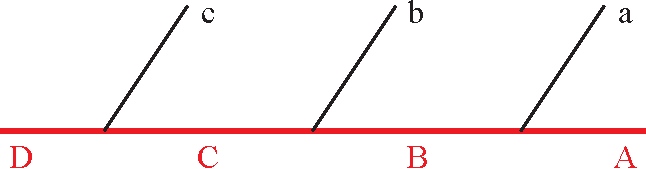
\includegraphics[scale=0.7]{figures/fig-chain.pdf} % Stolen!
\caption{Decay topology.}
\label{fig:decaytree}
\end{figure}

\section{Webber's method}
Webber \cite{Webber:2009vm} suggests a different method, where all kinematical info from every event is used. Consider the general decay tree in figure \ref{fig:decaytree}. Assuming that the decaying particles are on-shell, the 4-momenta in the upper chain should satisfy
\begin{align}
	(p_c + p_b + p_a + p_A)^2 &= M_D^2\nonumber \\
	(p_b + p_a + p_A)^2 &= M_C^2\nonumber \\
	(p_a + p_A)^2 &= M_B^2\label{eq:constraints}\\
	p_A^2 = M_A^2\nonumber
\end{align}
The first three equations give three linear constraints on the invisible 4-momentum $p_A$:
\begin{align}
	-2p_c\cdot p_A &= M_C^2 - M_D^2 + 2p_c\cdot p_b + 2p_c \cdot p_a + m_c^2 \equiv S_1,\nonumber \\
	-2p_b\cdot p_A &= M_B^2 - M_C^2 + 2p_b\cdot p_a + m_b^2 \equiv S_2,\\
	-2p_a\cdot p_A &= M_A^2 - M_B^2 + m_a^2 \equiv S_3. \nonumber
\end{align}
Equivalently the conjugate chain (with primed indices) gets the constraints
\begin{align}
	-2p_{c'}\cdot p_{A'} &= M_{C'}^2 - M_{D'}^2 + 2p_{c'}\cdot p_{b'} + 2p_{c'} \cdot p_{a'} + m_{c'}^2 \equiv S_5,\nonumber \\ 
	-2p_{b'}\cdot p_{A'} &= M_{B'}^2 - M_{C'}^2 + 2p_{b'}\cdot p_{a'} + m_{b'}^2 \equiv S_6,\\
	-2p_{a'}\cdot p_{A'} &= M_{A'}^2 - M_{B'}^2 + m_{a'}^2 \equiv S_7.\nonumber
\end{align}
In addition we have the transverse momentum constraints
\begin{align}
	p_A^x + p_{A'}^x &= p_\mathrm{miss}^x \equiv S_4, \label{eq:Svec_orig} \\
	p_A^y + p_{A'}^y &= p_\mathrm{miss}^y \equiv S_8. \nonumber
\end{align}

The vector $\mathbf{S} = (S_1, S_2, ...)$ thus depends on the eight unknown masses 
\begin{align}
	\mathbf{M} = (M_D^2, M_C^2, M_B^2, M_{A'}^2, M_{D'}^2, M_{C'}^2, M_{B'}^2, M_{A'}^2)
\end{align}
and the visible momenta which are measurable in principle. We define a vector containing the 4-momenta of the invisible final state particles as
\begin{align}
	\mathbf{P} = (p_A^x, p_A^y, p_A^z, E_A, p_{A'}^x, p_{A'}^y, p_{A'}^z, E_{A'}). \label{eq:Pvec}
\end{align}
We then have
\begin{align}
	\mathbf{A}\mathbf{P} = \mathbf{S},\label{eq:APS}
\end{align}
where
\begin{align}
	\mathbf{A} = 2 \begin{pmatrix}
						p_c^x & p_c^y & p_c^z & -E_c & 0 & 0 & 0 & 0 \\
						p_b^x & p_b^y & p_b^z & -E_b & 0 & 0 & 0 & 0 \\
						p_a^x & p_a^y & p_a^z & -E_a & 0 & 0 & 0 & 0 \\
						1/2 & 0 & 0 & 0 & 1/2 & 0 & 0 & 0\\
						0 & 0 & 0 & 0 & p_{c'}^x & p_{c'}^y & p_{c'}^z & -E_{c'} \\
						0 & 0 & 0 & 0 & p_{b'}^x & p_{b'}^y & p_{b'}^z & -E_{b'} \\
						0 & 0 & 0 & 0 & p_{a'}^x & p_{a'}^y & p_{a'}^z & -E_{a'} \\
						0 & 1/2 & 0 & 0 & 0 & 1/2 & 0 & 0
					\end{pmatrix}. \label{eq:Amatrix_orig}
\end{align}
Furthermore, $\mathbf{S}$ may be written as 
\begin{align}
	\mathbf{S} = \mathbf{B} \mathbf{M} + \mathbf{C},\label{eq:SBMC}
\end{align}
where
\begin{align}
	\mathbf{B} = \begin{pmatrix}
					-1 & 1 & 0 & 0 & 0 & 0 & 0 & 0 \\
					0 & -1 & 1 & 0 & 0 & 0 & 0 & 0 \\
					0 & 0 & -1 & 1 & 0 & 0 & 0 & 0 \\
					0 & 0 & 0 & 0 & 0 & 0 & 0 & 0 \\
					0 & 0 & 0 & 0 & -1 & 1 & 0 & 0 \\
					0 & 0 & 0 & 0 & 0 & -1 & 1 & 0 \\
					0 & 0 & 0 & 0 & 0 & 0 & -1 & 1 \\
					0 & 0 & 0 & 0 & 0 & 0 & 0 & 0 \\
	\end{pmatrix}
\end{align}
and
\begin{align}
	\mathbf{C} = ( &2p_c \cdot p_b + 2p_c \cdot p_a + m_c^2, 2 p_2 \cdot p_3 + m_b^2, m_a^2, p_\mathrm{miss}^x, \nonumber \\ 
				   &2p_{c'}\cdot p_{b'} + 2 p_{c'} \cdot p_{a'} + m_{c'}^2, 2 p_{b'} \cdot p_{a'} + m_{b'}^2, m_{a'}^2, p_\mathrm{miss}^y )
\end{align}
With all this, the solution for the invisible 4-momenta given the unknown masses is 
\begin{align}
	\mathbf{P} = \mathbf{A}^{-1} \mathbf{S} = \mathbf{D} \mathbf{M} + \mathbf{E}
\end{align}
where $\mathbf{D} = \mathbf{A}^{-1}\mathbf{B}$ and $\mathbf{E} = \mathbf{A}^{-1}\mathbf{C}$.

The matrix $\mathbf{D}$ and vector $\mathbf{E}$ contain only measurable quantities, hence they only need to be calculated once for every event. For the true value of the unknown masses $\mathbf{M}$, the system should satisfy the on-shell conditions
\begin{align}
	p_{A}^2 &= P_4^2 - P_1 ^2 - P_2^2 - P_3^2 = M_{A}^2, \nonumber\\
	p_{A'}^2 &= P_8^2 - P_5 ^2 - P_6^2 - P_7^2 = M_{A'}^2.
\end{align}
So by calculating $\mathbf{D}_n$ and $\mathbf{E}_n$ for each event $n$, and making a {\it hypothesis} $\mathbf{M}$ for the unknown masses, we can measure the goodness of fit for our hypothesis by the quantity
\begin{align}
	\xi^2(\mathbf{M}) = \sum_n \left[(p_{A}^2)_n - M_A^2\right]^2 + \left[(p_{A'}^2)_n - M_{A'}^2\right]^2. 
\end{align}
Note that this quantity measures the goodness-of-fit of all the unknown masses equally, since it follows from the constraint equations \eqref{eq:constraints} that {\it e.g.}
\begin{align}
	(p_B^2)_n - M_B^2 &= (p_a + p_A)_n^2 - M_B^2 = \nonumber\\
				  &= (p_a^2)_n + (p_A^2)_n + 2p_a\cdot p_A - M_B^2\nonumber\\
				  &= (p_a^2)_n + (p_A^2)_n - M_A^2 + M_B^2 - m_a^2 - M_B^2\\
				  &= (p_A^2)_n - M_A^2.\nonumber
\end{align}

The point of the method is to minimize $\xi^2$ as a function of $\mathbf{M}$. This is generally an eight-dimensional minimization problem with a very complicated function, and thus not easy to solve. However, in the case of identical chains, it reduces to a much more handleable four-dimensional one. The condition of identical chains can often be satisfied by a combination of vetoing ({\it e.g.} b-jets) and assuming small mass splittings between different generations, thus approximating their masses as equal. 

\section{Making sense of dimensions}\label{sec:dimension_fixing}
The aptness of the method hangs on the invertibility of the matrix $\mathbf{A}$. However, the matrix as it stands in \eqref{eq:Amatrix_orig}, is ill-defined for inversion since not all rows have the same units. The rows 4 and 8, corresponding to the components 4 and 8 of the vector $\mathbf{S}$ \eqref{eq:Svec_orig}, have no dimension, while the other rows have dimension $(\mathrm{mass})^1$. This is reflected in the components of $\mathbf{S}$, which all except 4 and 8 have dimension $(\mathrm{mass})^2$. This means both that the magnitude of the determinant is sensitive to the choice of mass scale (since some rows have non-zero dimension) and that it does not scale properly (since not all rows have the same dimension). This is something that Webber does not comment on, but we take steps to amend both problems.

For the first, we redefine $S_4$ and $S_8$ to be 
\begin{align}
	S_4 &\equiv (p_A^x + p_{A'}^x)^2 = (p_\mathrm{miss}^x)^2, \label{eq:Svec_modified} \\
	S_8 &\equiv (p_A^y + p_{A'}^y)^2 = (p_\mathrm{miss}^y)^2. \nonumber
\end{align}
We do not wish to redefine $\mathbf{P}$ \eqref{eq:Pvec}, so to keep the relationship $\mathbf{S} = \mathbf{A}\mathbf{P}$ we modify rows 4 and 8 of $\mathbf{A}$ to
\begin{align}
	\mathbf{A}_4 &= (p_\mathrm{miss}^x, 0, 0, 0, p_\mathrm{miss}^x, 0, 0, 0),\\
	\mathbf{A}_8 &= (0, p_\mathrm{miss}^y, 0, 0, 0, p_\mathrm{miss}^y, 0, 0),\nonumber
\end{align}
such that $\mathbf{A}$ now is
\begin{align}
	\mathbf{A} = 2 \begin{pmatrix}
						p_c^x & p_c^y & p_c^z & -E_c & 0 & 0 & 0 & 0 \\
						p_b^x & p_b^y & p_b^z & -E_b & 0 & 0 & 0 & 0 \\
						p_a^x & p_a^y & p_a^z & -E_a & 0 & 0 & 0 & 0 \\
						p_\mathrm{miss}^x/2 & 0 & 0 & 0 & p_\mathrm{miss}^x/2 & 0 & 0 & 0\\
						0 & 0 & 0 & 0 & p_{c'}^x & p_{c'}^y & p_{c'}^z & -E_{c'} \\
						0 & 0 & 0 & 0 & p_{b'}^x & p_{b'}^y & p_{b'}^z & -E_{b'} \\
						0 & 0 & 0 & 0 & p_{a'}^x & p_{a'}^y & p_{a'}^z & -E_{a'} \\
						0 & p_\mathrm{miss}^y/2 & 0 & 0 & 0 & p_\mathrm{miss}^y/2 & 0 & 0
					\end{pmatrix}. \label{eq:Amatrix_modified}
\end{align}

This redefinition does not alter the solvability of the problem, since the only information lost in $\mathbf{S}$ is the sign of $p_\mathrm{miss}^i$ which is kept in $\mathbf{A}$ instead. Also it keeps the essential feature that $\mathbf{A}$ only contains measured quantities, such that it can be inverted prior to making a mass hypothesis. The redefinition of $\mathbf{S}$ means we also have to modify $\mathbf{C}$ to keep the relationship $\mathbf{S} = \mathbf{B} \mathbf{M} + \mathbf{C}$ (Eq. \eqref{eq:SBMC}). We thus make the same redefinitions here, {\it i.e.}
\begin{align}
	C_4 &\equiv (p_\mathrm{miss}^x)^2, \label{eq:Cvec_modified} \\
	C_8 &\equiv (p_\mathrm{miss}^y)^2. \nonumber
\end{align}

The other problem was to make the mathematics dimensionless. All elements of $\mathbf{A}$ and $\mathbf{P}$ now have mass dimension 1, while all elements of $\mathbf{S}$, and thus $\mathbf{M}$ and $\mathbf{C}$, have dimension 2. We are free to multiply both sides of Eq. \eqref{eq:APS} by some normalization mass $M_\mathrm{norm}$ squared,
\begin{align}
	\frac{1}{M_\mathrm{norm}^2} \mathbf{A}\mathbf{P} = \frac{1}{M_\mathrm{norm}^2} \mathbf{S},
\end{align}
and we choose to take it into the matrix and vectors such that they all become dimensionless, {\it i.e.}\ we modify
\begin{align}
	\mathbf{\hat A} = \frac{1}{M_\mathrm{norm}}\mathbf{A},\nonumber \\
	\mathbf{\hat P} = \frac{1}{M_\mathrm{norm}}\mathbf{P},\label{eq:vectors_normalized}\\
	\mathbf{\hat S} = \frac{1}{M_\mathrm{norm}^2}\mathbf{S},\nonumber 
\end{align}
thus modifying $\mathbf{M}$ and $\mathbf{C}$ in the same way as $\mathbf{S}$ to comply with Eq. \eqref{eq:SBMC}. We also modify the fitting function $\xi^2$ accordingly, so that it becomes
\begin{align}
	\xi^2(\mathbf{M}) = \sum_n \left[(\hat p_{A}^2)_n - \frac{M_A^2}{M_\mathrm{norm}^2}\right]^2 + \left[(\hat p_{A'}^2)_n - \frac{M_{A'}^2}{M_\mathrm{norm}^2}\right]^2.
\end{align}

To obtain numbers of order 1, which is optimal for numerical purposes, we should pick a mass of the relevant scale for the problem. This is not something that is known {\it \`a priori}, since it depends on the supersymmetric masses that we are trying to determine. We might be tempted to use something based on the measured momenta, but this is a bad idea since it would mean weighting different events differently. We choose the normalization constant
\begin{align}
	M_\mathrm{norm} = 1 \,\mathrm{TeV},
\end{align}
the characteristic energy scale of electroweak processes.

\section{Outline of the plan}
In this thesis we wish to investigate and hopefully develop this method further. We will begin by reproducing Webber's parton level results using Monte Carlo simulations. We will then add layers of realism and complexety approaching something closer to the real experimental situastion, in order to investigate its full potential. In the end we will focus on well motivated scenarios that can be discovered in Run II of the LHC.  Along the way we will also make some improvements on the method.

The plan of attack is as follows:
\begin{enumerate}
	\item We begin by generating squark pairs at 14 TeV using {\tt CompHEP}, decaying them in the chain of on-shell two-body decays given in (\ref{eq:goldencascade}). The visible decay products, quarks and leptons, are then used to reconstruct the masses. As a benchmark we investigate the precission atainable for the parameter point SPS1a~\cite{Allanach:2002nj}. 
	\item	We then compare results with and without including the combinatorical issues from identifying the decay products, and we add a simple parametrised momentum smearing, based on realistic detector response, in order to simulate that the measurement of the kinematics of final-state particles is not exact. This was the level of precission employed by Webber in~\cite{Webber:2009vm}.
	\item Because of final state radiation and parton showering, as well as---to a lesser degree---sparticle widths, the particles in the decay chain will not be on-shell due to extra gluons (and photons) in the final state. We employ a more sophisticated Monte Carlo code, {\tt Herwig++}~\cite{Bahr:2008pv}  to simulate these properties. This should have an effect on the mass reconstruction since Webber's method assumes on-shell decays.
	\item The partons that emerge from the hadron showers will hadronize, forming a hadron jet before arriving in the detector. Measurement of the initial parton from reconstructing such jets is one of the big challenges of collider physics. We use the {\tt FastJet}~\cite{Cacciari:2011ma} program for jet reconstruction, with algorithms used in the LHC experiments, and study the effect of jet reconstruction on the mass measurement.
	\item In an analysis of real data, one would have to use selection criteria such as cuts on transverse momentum and number of jets and leptons to discriminate between signal and background events. We will apply such cut schemes to our simulated events based on expectations for 14 TeV LHC. In addition we simulate the expected largest backgrounds for a four-lepton supersymmetry search and investigate how the performance of the method is affected by the presence of background.
	\item {\bf If time} As a last step towards realism, we put the events through a fast detector simulation. 
	\item We then investigate improvements over the original model. Webber and collaborators \cite{Nojiri:2010dk} propose combining the kinematical best-fit reconstruction with measurements of end points of invariant mass distributions.
	\item Investigating other types of chains. Not-equal-sided? Different number of steps? Fitting a mass plane rather than points?
	\item Finally, we look at a well motivated model taken from \cite{Allanach:2014gsa} that was constructed on the basis of a small excess seen in 8 TeV data by the CMS Collaboration~\cite{CMS:2014jfa}, which would be consistent with the decay chain in (\ref{eq:goldencascade}). We show what precission we can expect from mass measurments at 14 TeV LHC should such a scenario be realized.
\end{enumerate}







%%%%%%%%%%%%%%%%%%%%%%%%%%%%%%%%%%%%%%%%%%%%%%%%%
\chapter{Investigating Webber's method by Monte Carlo simulation}
\label{ch:MC}
%%%%%%%%%%%%%%%%%%%%%%%%%%%%%%%%%%%%%%%%%%%%%%%%%
Webber demonstrates the aptitude of the method on a Monte Carlo generated dataset. We wish to reproduce his results. 

\section{Production mechanisms}
There are several ways in which a pair of squarks can be produced in $pp$ collisions. Figure \ref{fig:squark_production_diagrams} shows Feynman diagrams of different processes that contribute.\footnote{The diagrams are made using JaxoDraw \cite{Binosi:2003yf}.} In (a) and (c) the squarks are opposite sign and in (a) also same flavour, while in (b) and (d) we have no such guarantee. Additionally, in (b) and (d) the squarks are produced along with additional quarks.

\begin{figure}[hbt]
	\centering
	\begin{subfigure}[b]{0.4\textwidth}
		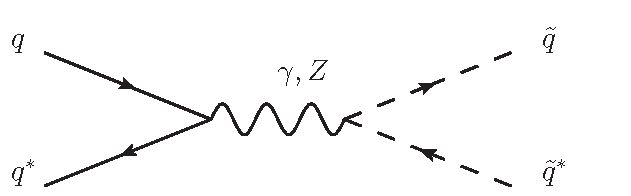
\includegraphics[width=\textwidth]{figures/qqbar_to_tildeqqbar_s_channel.pdf} 
		\caption{ }
	\end{subfigure}
	\begin{subfigure}[b]{0.4\textwidth}
		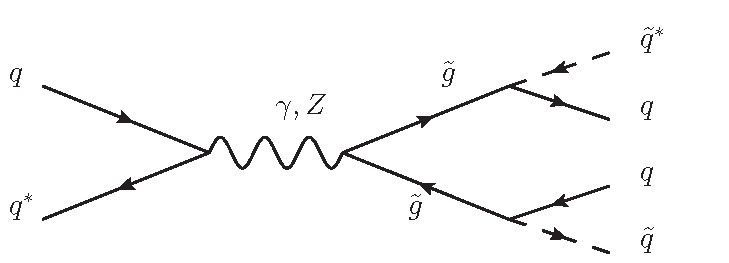
\includegraphics[width=\textwidth]{figures/qqbar_to_gluinos_to_qqtildeqq_s_channel.pdf}
		\caption{ } 
	\end{subfigure}

	\begin{subfigure}[b]{0.4\textwidth}
		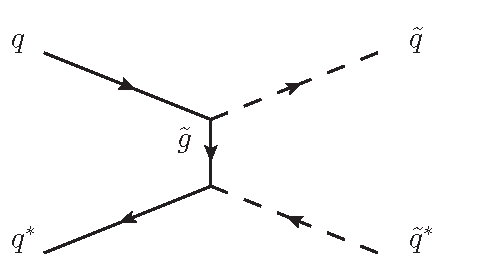
\includegraphics[width=\textwidth]{figures/qqbar_to_tildeqqbar.pdf} 
		\caption{ }
	\end{subfigure}
	\begin{subfigure}[b]{0.4\textwidth}
		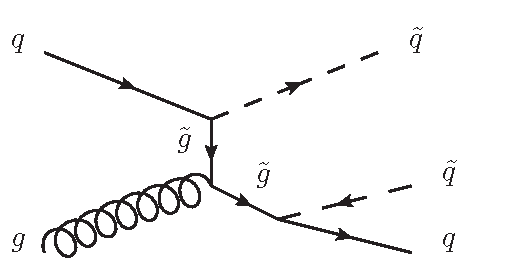
\includegraphics[width=\textwidth]{figures/qg_to_tildeqqbar.pdf}
		\caption{ } 
	\end{subfigure}
	\caption{Diagrams for squark pair production.}
	\label{fig:squark_production_diagrams}
\end{figure}

However, the production of additional quarks is irrelevant for the analysis and reconstruction of the cascade, because we only wish to reconstruct the chain back to the squark. So is the distinction between squark flavours. The only significance of the flavour of squark is on the flavour of quark it decays to along with the $\chi_2^0$ -- the quark and squark must be of the same flavour and sign. The $\chi_2^0$ cannot transmit any information about the flavour of its squark mother, so the subsequent leptonic decay is independent of the previous history. The quark will hadronize to form a hadron jet, and the properties of this jet are in principle dependent on the type of quark. However, current detectors are not good at discriminating between quark flavours of the first two generations; it can only discover $b$ quarks using the technique of {\it b-tagging} and to some extent $c$ quarks via {\it c-tagging}. In our analysis we will veto events containing $b$ quarks as the mass splitting of the squarks between the first/second and third generation prevent a good fit with a single squark mass.




\section{Event generation using {\tt CompHEP}}
We first begin by using {\ttfamily CompHEP 4.5.2} \cite{Pukhov:1999gg} to generate 1000 $pp \to \tilde{u}_L \bar{\tilde{u}}_L$ collisions at $\sqrt{s} = 14 \, \mathrm{TeV}$ with the supersymmetric parameter choice mSUGRA SPS1a $(\alpha)$ \cite{Allanach:2002nj} calculated using {\ttfamily SoftSUSY 3.4.1} \cite{Allanach:2001kg}.\footnote{Note that CompHEP uses the wrong squark mass: The value from SoftSUSY is $\sim 565 \,\mathrm{GeV}$, while CompHEP uses $\sim 545 \,\mathrm{GeV}$. This is due to how CompHEP is coded: The external RGE running done by SoftSUSY is only used by CompHEP up to the point of low-scale soft mass parameters. The calculation of physical squark masses from soft mass parameters is hard-coded in CompHEP using a tree-level formula. Trying to manually change the value has proven difficult since it disturbs the internal consistency of CompHEP.} \marginpar{TODO: Make CompHEP use the correct squark mass if possible.} {\ttfamily CompHEP} produces a file containing the 4-momenta of the squarks for each event. It is important to note that {\ttfamily CompHEP} produces the squarks on-shell -- possibly a major simplification for colour-charged particles, who might realistically be far off-shell when they come from a hard collision before they have a chance to shower off gluons. The squark 4-momenta are then read into a Python script where the rest of the chain is generated. We generate the chain as a succession of two-body decays where the decay products are on-shell, {\it e.g.}\ we work in a narrow width approximation. This is again a major simplification for the quark due to showering. Standard model particles are assumed massless. The algorithm for this generation is described in section \ref{sec:decayalgorithm}. The decay direction for the back-to-back decay in each step is drawn uniformly on a sphere. This is correct for the scalar particles, and for the fermions it is justified by averaging over spin directions. \marginpar{\color{purple} Note to self: Check that I understand this properly.} The resulting visible 4-momenta resemble an idealized decay situation. As a check to see that our algorithm is correct, we reproduce the dilepton invariant mass distribution for the upper chain as discussed in the previous section. The distribution is shown in figure \ref{fig:dilepton_invariant_mass_no_smearing}. We see that it resembles a triangle, and that it cuts sharply at $m_{ll}^{\mathrm{max}} \approx 80 \, \mathrm{GeV}$, which corresponds nicely with the theoretical prediction $m_{ll}^\text{max} = 80.2 \, \mathrm{GeV}$ from Eq. \ref{eq:invariant_mass_endpoint}.

\begin{figure}[hbt]
\centering
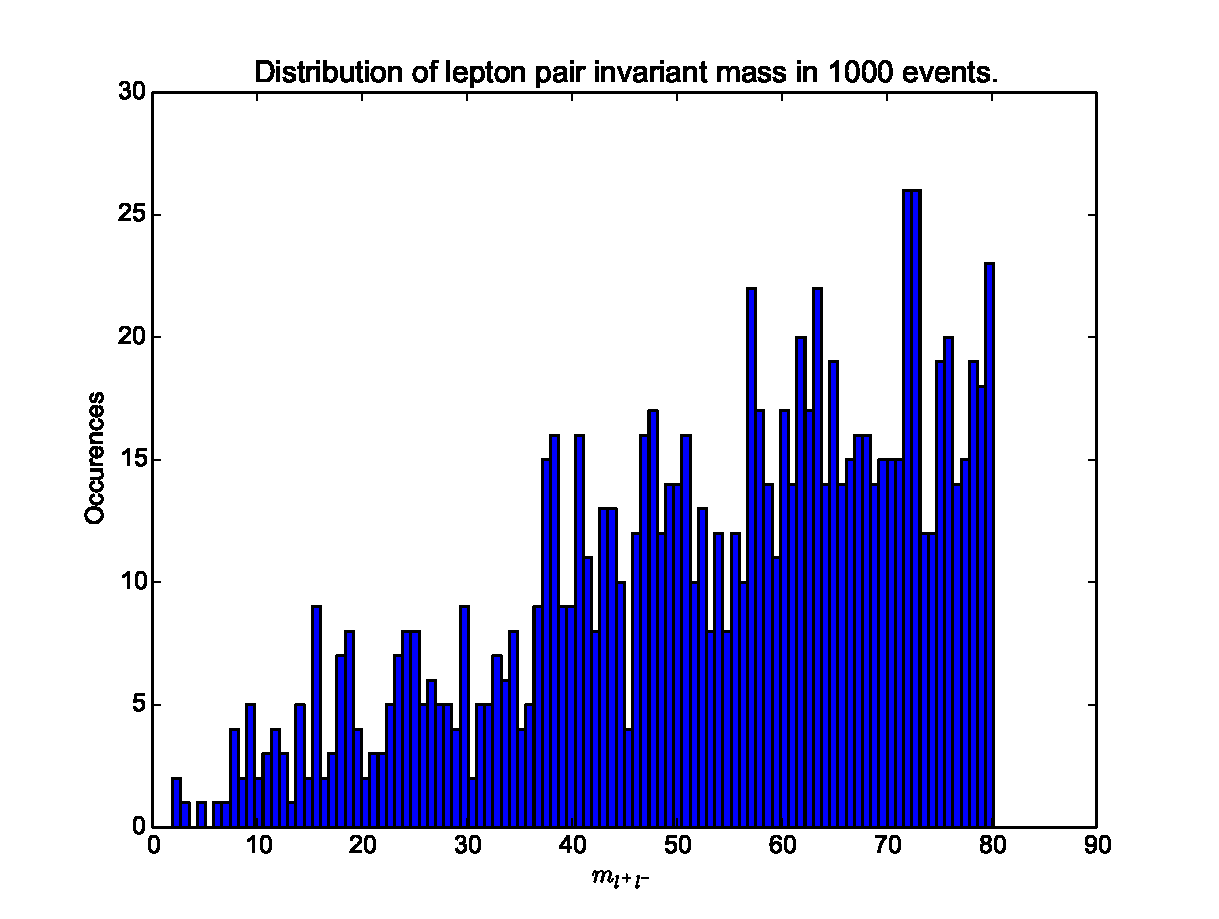
\includegraphics[scale=0.7]{figures/dilepton_invariant_mass_comphep-data_smearing-0_events-1000.pdf} 
\caption{Dilepton invariant mass distribution.}
\label{fig:dilepton_invariant_mass_no_smearing}
\end{figure} \marginpar{Redo dilepton invmass plot with fewer bins and larger font. Also change colour?}



\section{$\xi^2$ minimization}
\marginpar{This paragraph is up for deletion.}
{\color{gray} We also test the mass reconstruction method on this idealized dataset. Webber uses the {\ttfamily MINUIT} algorithm {\ttfamily SIMPLEX}, which we also apply. We use it in the form of the python package {\ttfamily PyMinuit} \cite{PyMinuit,James:1975dr}. Applying {\ttfamily SIMPLEX} to the method, using the entire dataset of 1000 events, gives excellent results -- way too good to be realistic, as we might anticipate, given the high level of idealization and large number of events. Data from fitting 1000 events is shown in table \ref{table:fit_no_smear}. We see that the error in the fit is at the level of a few percent.}
\marginpar{Note: The mass used for generation is the comphep-wrong one. Should redo with proper mass if I can fix the problem.}

\begin{table}[hbt]
	\centering
	\begin{tabular}{| l | l | l | l | l |}
		\hline
							&  $m_{\tilde{q}}$ & $m_{\tilde{\chi}_2^0}$ & $m_{\tilde{l}}$ & $m_{\tilde{\chi}_1^0}$ \\ \hline
		True values [GeV] 	& 545.4 & 180.3 & 144.1 & 97.0 \\ \hline
		Best-fit values [GeV] & 546.8 & 184.2 & 148.9 & 104.0 \\ \hline
		Relative fit error  & 0.2 \% & 2.1 \% & 3.3 \% & 7.2 \% \\ \hline
	\end{tabular}
	\caption{SIMPLEX fit of 1000 events in an idealized situation.}
	\label{table:fit_no_smear}
\end{table}

We split the events in 25 event bins and apply the method to each bin. For the minimization we employ {\ttfamily SciPy} \cite{SciPy} with TNC \cite{Nash:1984}. We try several choices for the initial parameter guess, to investigate how different starting points affect minimization performance.

\begin{table}[hbt]
	\centering
	\begin{tabular}{| l | l | l | l | l |}
		\hline 
		x $\backslash$ Particle   			& $\tilde q$ 	&$\tilde \chi_2^0$ 	& $\tilde l$ 	& $\tilde \chi_1^0$    	\\ \hline
		True mass [GeV]     & 568 (average) & 180				& 144			& 97					\\
		1.1 &	$570 \pm 15 [29]$ & $196 \pm 5 [17]$ & $159 \pm 4 [15]$ & $111 \pm 6 [16]$ \\
		0.9 &	$526 \pm 16 [25]$ & $166 \pm 5 [15]$ & $130 \pm 3 [15]$ & $80 \pm 6 [18]$ \\
		0.5 &	$445 \pm 75 [123]$ & $118 \pm 24 [67]$ & $84 \pm 17 [62]$ & $28 \pm 20 [72]$ \\
		2.0 &	$824 \pm 184 [334]$ & $334 \pm 37 [159]$ & $285 \pm 24 [143]$ & $221 \pm 34 [129]$ \\ \hline
	\end{tabular}
	\caption{Summary of TNC fits to 25 event bins corresponding to figure \ref{fig:comphep_scipy_TNC_fits}. Fitted parameters are given as `average over bins $\pm$ empirical rms variation [true rms variation]'. The true rms variation means rms deviation from the true mass value rather than the mean. The $x$'s are defined such that $M_\mathrm{initial}= x M_\mathrm{true}$ for all unknown masses, $M_\mathrm{initial}$ being the starting point of the search.}
	\label{table:comphep_scipy_TNC_fits}
\end{table}

\begin{figure}[hbt]
	\centering
	\begin{subfigure}[b]{0.49\textwidth}
		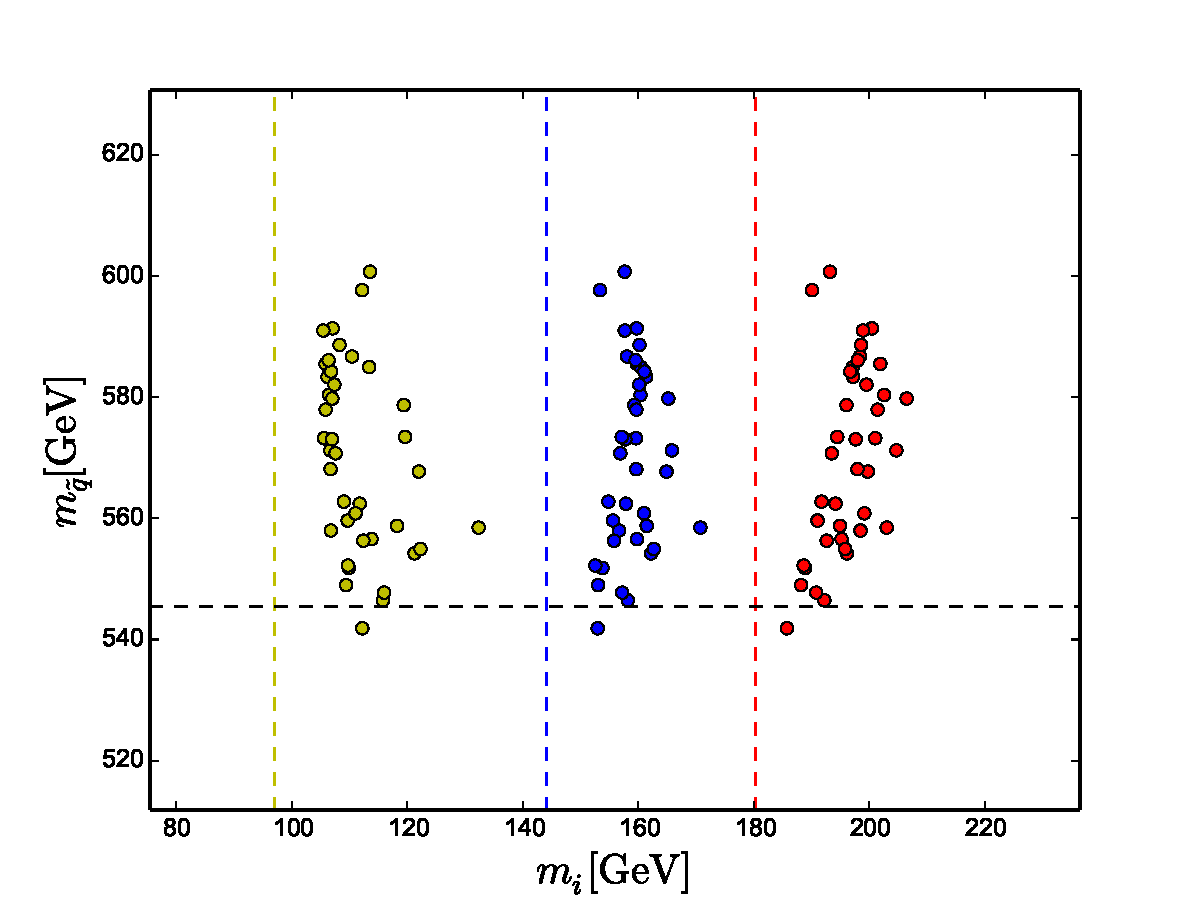
\includegraphics[width=\textwidth]{figures/comphep_scipy_TNC_fit_1p1_initial_guess.pdf} 
		\caption{}
		\label{fig:comphep_scipy_TNC_fits1}
	\end{subfigure}
	\begin{subfigure}[b]{0.49\textwidth}
		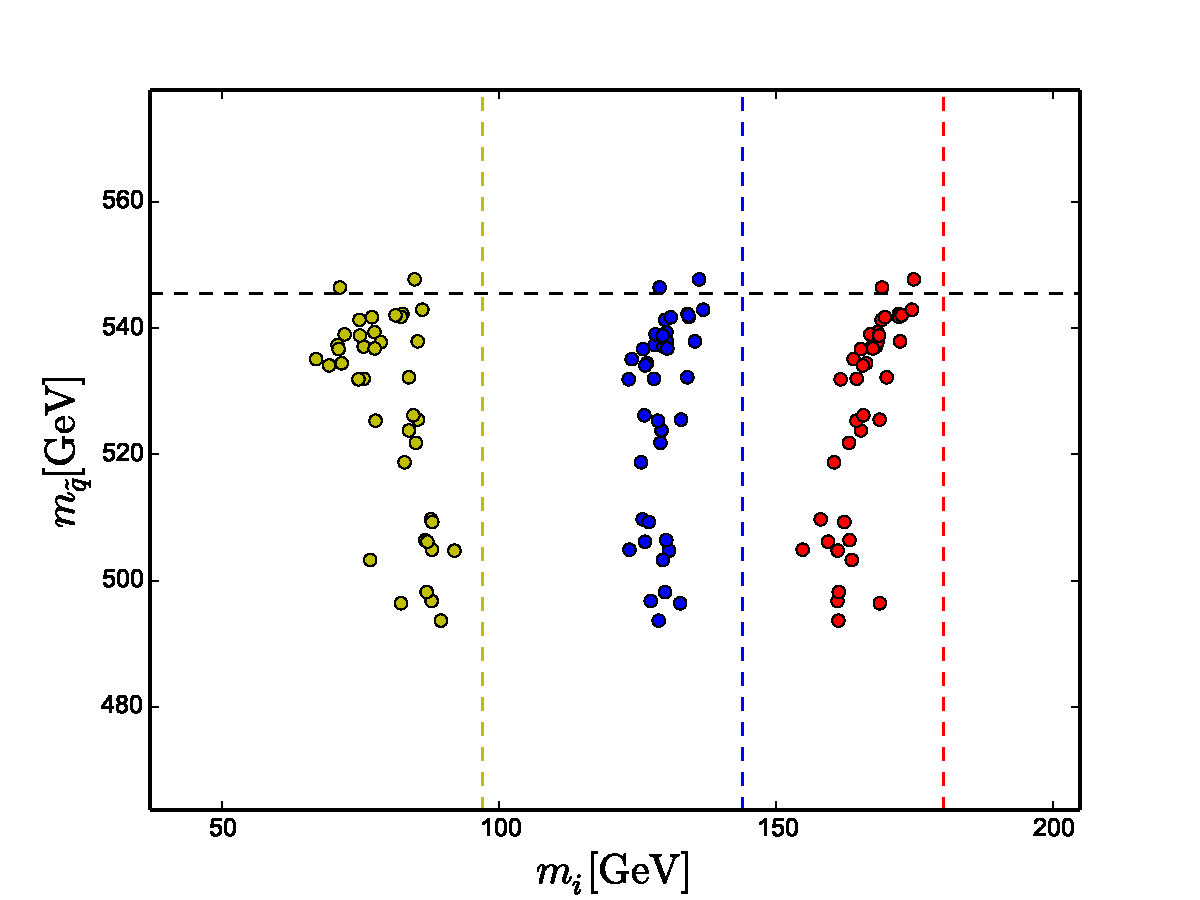
\includegraphics[width=\textwidth]{figures/comphep_scipy_TNC_fit_0p9_initial_guess.pdf} 
		\caption{}
		\label{fig:comphep_scipy_TNC_fits2}
	\end{subfigure}

	\begin{subfigure}[b]{0.49\textwidth}
		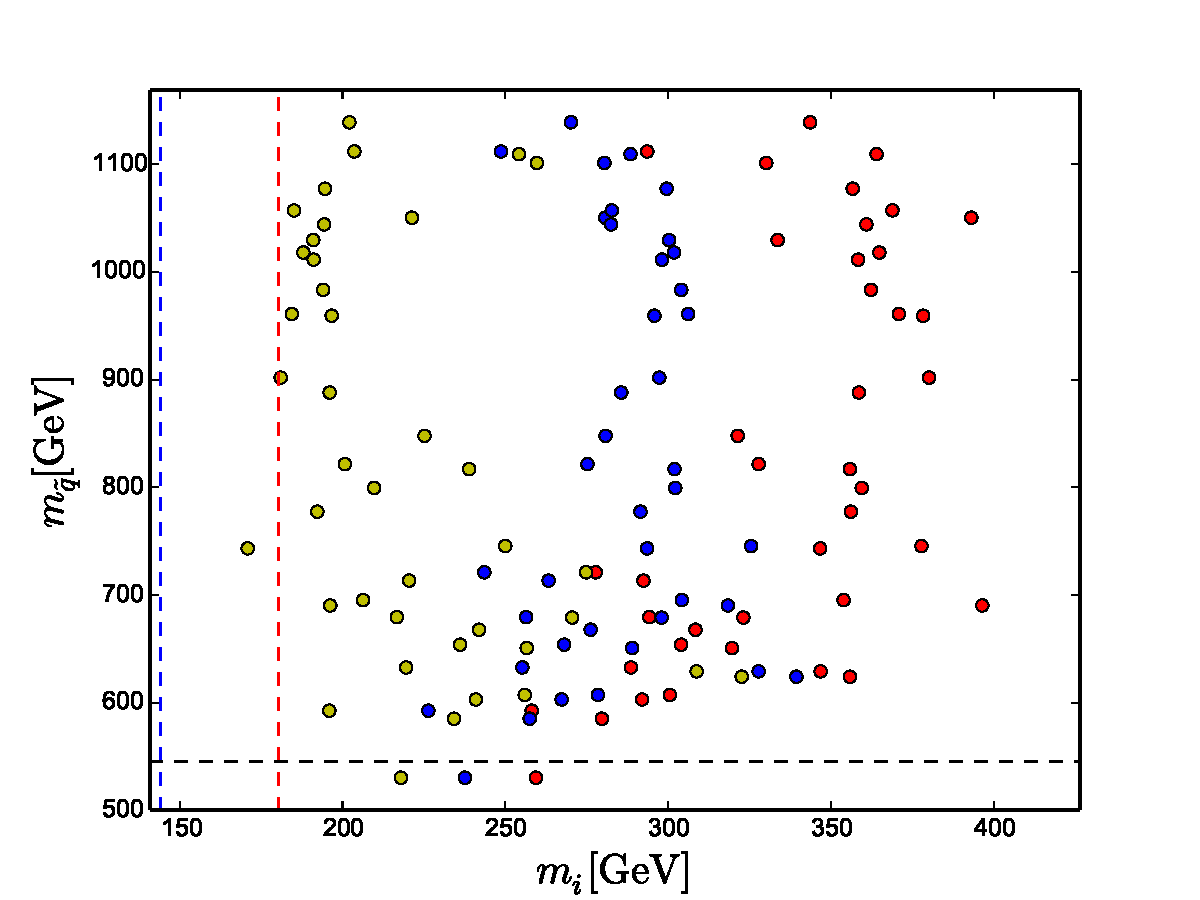
\includegraphics[width=\textwidth]{figures/comphep_scipy_TNC_fit_2p0_initial_guess.pdf} 
		\caption{}
		\label{fig:comphep_scipy_TNC_fits3}
	\end{subfigure}
	\begin{subfigure}[b]{0.49\textwidth}
		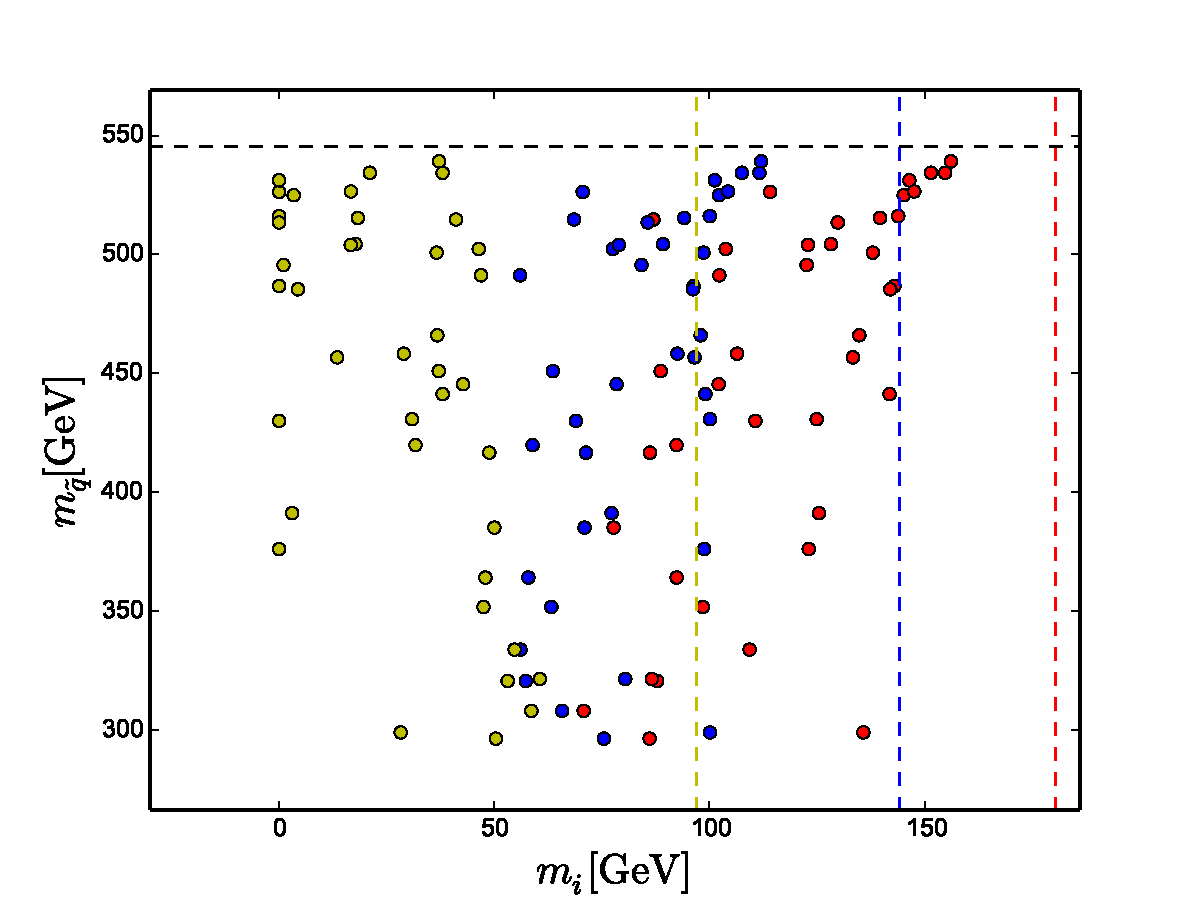
\includegraphics[width=\textwidth]{figures/comphep_scipy_TNC_fit_0p5_initial_guess.pdf} 
		\caption{}
		\label{fig:comphep_scipy_TNC_fits4}
	\end{subfigure}
	\caption{Best-fit points for 40 bins of 25 CompHEP generated events minimized with TNC, with different initial parameter guesses $M_\mathrm{initial} = x M_\mathrm{true}$, where $x = 1.1$ for (a), 0.9 for (b), 2.0 for (c) and 0.5 for (d). The points are summarized in table \ref{table:comphep_scipy_TNC_fits}.}
	\label{fig:comphep_scipy_TNC_fits}
\end{figure} 




\section{The effects of sorting out dimensions}\marginpar{Note: Consider dropping this section entirely? Or at least redo it with binning, with correct datasets, etc.}
It is interesting to see whether our modifications of Webber's mathematics, discussed in section \ref{sec:dimension_fixing}, have any effect on computation time, accuracy or even whether {\ttfamily SIMPLEX} finds the minimum at all. We did a test of this, using 25 of the {\ttfamily CompHEP} events and running through the different smearings $s= 0,0.5,1,3,6$ and $10$. For the basic formulation without the dimension fixing and without normalizing, the {\ttfamily SIMPLEX} routine fails to find the minimum even for zero smearing. Normalizing the $\xi^2$ function by the number of events helps to make it past zero smearing and 0.5 smearing, but then it fails. For zero smearing the mean absolute relative fit error compared to the true masses is at the order of $10^{-7}$. Running with the dimensions of $\mathbf{A}$ fixed according to Eq. \eqref{eq:Amatrix_modified} also fails beyond 0.5 smearing, and the error even for 0 smearing is actually increased to the order of $10^{-2}$. By also including the normalization as given in Eqs. \eqref{eq:vectors_normalized}, the script runs through all smearings and manages to get a fit in every case. We note that the error in this fully dimensionless implementation is of the order $10^{-2}$ for 0 smearing, thus actually higher than for the original implementation. This is however only for one 25 event sample, and should be studied more carefully before drawing conclusions. The total run time for the dimensionless fit is a couple of seconds. By mistake we discovered that dividing the $\xi^2$ by a number of order $10^8$ actually decreased computation time further, by about a factor 2. This indicates that {\ttfamily SIMPLEX} prefers to work with small numbers, at least in the {\ttfamily PyMinuit} implementation.



\section{Switching to a more sophisticated event generator: {\ttfamily Herwig++}}
% Even with smearing, we get a reconstruction that is much better than Webber. 
In our fit thus far, we have used events generated by {\ttfamily CompHEP} at squark level and decayed them in a very basic way. One obvious flaw in our model is the lack of {\it parton showering}---the radiation of gluons (and in turn quarks and antiquarks) emitted from the quark in the squark to quark decay process. If showering is taken into account, it means that the initial quark in the squark two-body decay can be off-shell, since it is really carrying the energy and momentum of not only itself, but also (several) other partons.\footnote{This statement should not be taken too literally, since the showering of a discrete number of gluons is just an approximate model of the re-summed contribution from higher-order diagrams in perturbation theory.}

To this end we employ {\ttfamily Herwig++  2.7.1}~\cite{Bahr:2008pv} for Monte Carlo event generation. This is a complete simulation code for particle collisions, generating hard parton processes from parton distribution functions, handling decays, including (s)particle widths and mass smearing according to Breit-Wigner distributions, initial and final state radiation including parton showering, multiple interactions {\it etc}. The user has access to all the information from each event though a {\ttfamily C++} analysis function that can be linked as a library and run by {\ttfamily Herwig++} for each event.

\subsection{{\ttfamily Herwig++} setup}

We continue to simulate $pp$ collisions at $\sqrt{s}=14 \, \mathrm{TeV}$. For the following, we turn off the hadronization module in {\ttfamily Herwig++}---treating quarks and gluons as final state particles. 
%We have to enter a list of the partons that we wish to be able to collide -- we choose $u,d,c,s$ and $g$ plus their antiparticles. 
We generate sparticle pair production, with the first two generations of left-handed squarks: $\tilde{u}_L,\tilde{d}_L,\tilde{c}_L$ and $\tilde{s}_L$ plus their antiparticles. The exclusion of third-generation squarks from the analysis is done because the difference in masses prevents a good fit under the assumption of a single squark mass. At SPS1a, there is mass degeneracy between left-handed squarks of up- and down-type respectively, for the first two generations. The masses are $m_{\tilde u_L, \tilde c_L} = 565 \,\mathrm{GeV}$ and $m_{\tilde d_L, \tilde s_L} = 571 \, \mathrm{GeV}$, {\it i.e.}\ the mass splitting $\Delta m = 6 \, \mathrm{GeV}$ is small. 

We use only left-handed squarks because the production of $\tilde \chi_2^0$ from right handed squarks is small---at SPS1a the 2nd generation neutralino is mostly wino whilst the 1st generation is mostly bino, and the wino only couples to left-handed squarks. For instance, the branching ratio for $\tilde u_R \to u \tilde \chi_2^0$ is $\sim 1 \%$, whilst for $\tilde u_L$ it is $\sim 30 \%$. The exclusion of events with unwanted squarks is done in the post-generation analysis.

Futhermore, the mass hierarchy of SPS1a is such that the left-handed sleptons $\tilde e_L, \tilde \mu_L$ are heavier than $\chi_2^0$, thus disabling those decay modes for the $\chi_2^0$. Since first- and second generation sleptons of the same chirality are mass-degenerate at this parameter point, it means that we only have one slepton mass to fit.

The choice of MSSM parameters is input into {\ttfamily Herwig++} using an SLHA model file~\cite{Skands:2003cj} for the SPS1a parameter point
%{\ttfamily MadGraph} \cite{Alwall:2014hca}
generated by {\ttfamily SoftSusy 3.4.1}~\cite{Allanach:2001kg} and post-processed by {\ttfamily SUSY-HIT 1.4} \cite{Djouadi:2006bz} to calculate branching ratios. We disable all decay channels except those that produce our chain (\ref{eq:goldencascade}). 

\subsection{Herwig++ event analysis routine} 

A few technical aspects of the per-event analysis done with {\ttfamily Herwig++} should be mentioned. Even though we have disabled all but the relevant decay modes in the simulation, {\ttfamily Herwig++} resets some of the other branchings to small, nonzero values. This means that we must check each event to see that it really contains two instances of the correct cascade. This is done in an analysis routine linked by the {\ttfamily Herwig++} run. At each decay vertex we check that the PDG codes of the outgoing particles match what we expect.

{\ttfamily Herwig++} showers the squarks and quarks. In the showering process it will make several instances of the same particle, {\it e.g.}\ the quark, where the subsequent instances are in a mother-daughter relationship among the event particles. Care has to be taken to ensure that we pick the correct instance of the quark, and we have done tests of momentum conservation to check that we indeed pick the right instance.

There is also the possibility of photon bremsstrahlung in the other charged particle decays, {\it i.e.}\ the $\tilde \chi_2^0$ and $\tilde l$. This is treated as an $N$-body decay in {\ttfamily Herwig++}, with two massive decay products and $N-2$ photons. We allow these events past our vetoes, and discard the photons -- thus introducing an inaccuracy in the momentum conservation -- on the basis that they would be difficult to identify in a detector event. \marginpar{Note: Here we have the option in the code to veto events with large photon momenta. Should we pursue it?}


\subsection{Parton showering}
The distribution of quark invariant masses prior to their showering off gluons are shown in figure \ref{fig:invmass_offshellquarks}.

\begin{figure}[hbt]
\centering
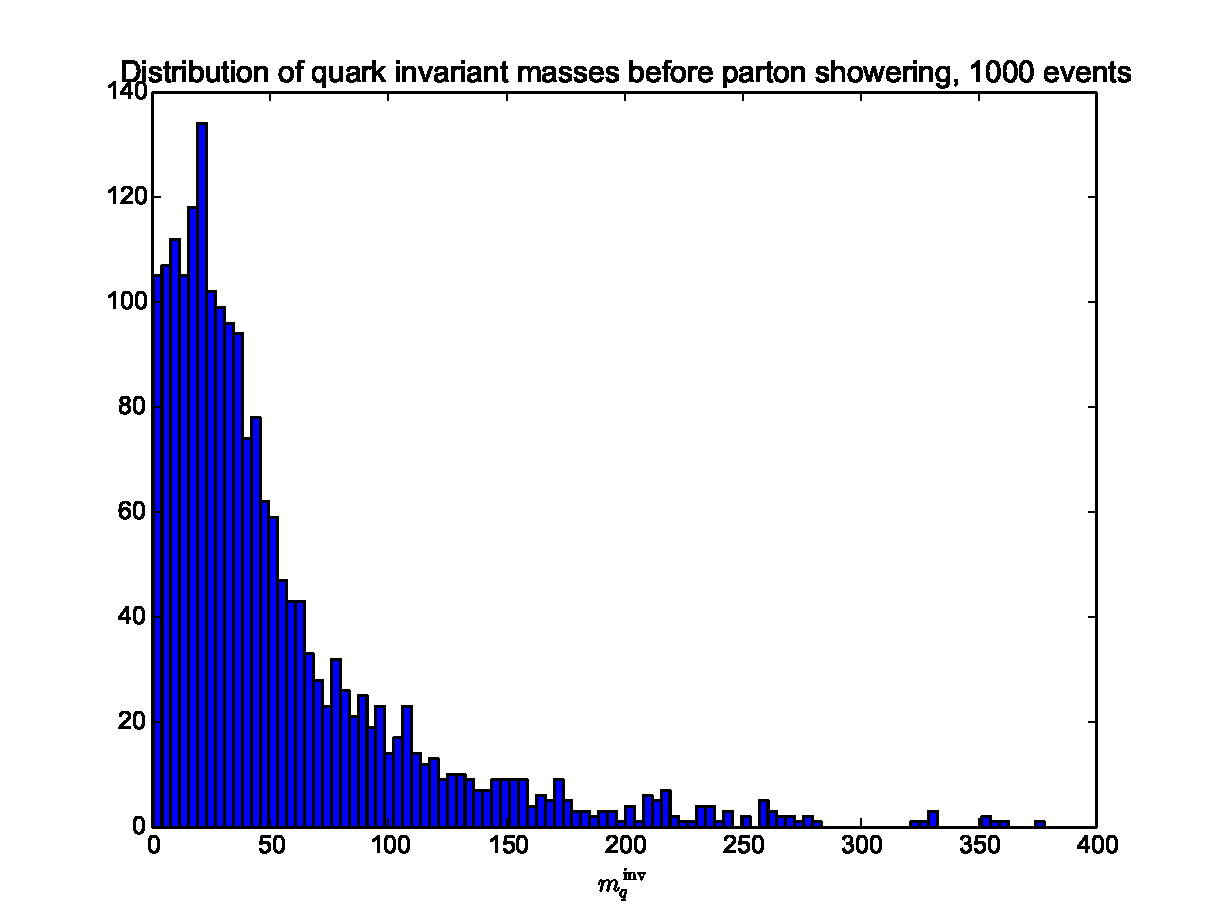
\includegraphics[scale=0.7]{figures/quark_invmass_before_showering_both_chains_combined_N1000.pdf} 
\caption{Invariant mass distribution of offshell quarks from squark decays. Quarks from both chains in 1000 {\ttfamily Herwig++} generated events are shown. Quark flavours are $u,d,c$ and $s$.}
\label{fig:invmass_offshellquarks}
\end{figure}

\subsection{Fitting the {\ttfamily Herwig++} events}
The $\xi^2$ function is quartic in the four unknown masses. Without taking combinatorical ambiguities into account, it has a smooth surface and a well-defined minimum. Figure \ref{fig:3D_masses} shows the $\log(\xi^2)$ surface as a function of pairs of masses. Notice that the minimum is significantly less pronounced for $m_{\chi_2^0}$ than for the other three masses. Subfigure (d) shows a rotated view to illustrate this. The plotting limits for each mass is from $0.5$ to $1.5$ of the minimum, so it means that the steepness of $\xi^2$ relative to the lightest mass is less than the others. This may mean that it is more difficult to fit this mass than the others, which is consistent with our earlier speculations and with the rms errors in table \ref{table:herwig_migrad_nosmear_1p01} -- more on that in a moment. It will be interesting to see how combinatorics affects this. \marginpar{Note to self: Or could this be the result of Migrad not finding a better guess than the initial value for the OTHER masses in many of the bins?}





\begin{figure}[hbt]
	\centering
	\begin{subfigure}[b]{0.49\textwidth}
		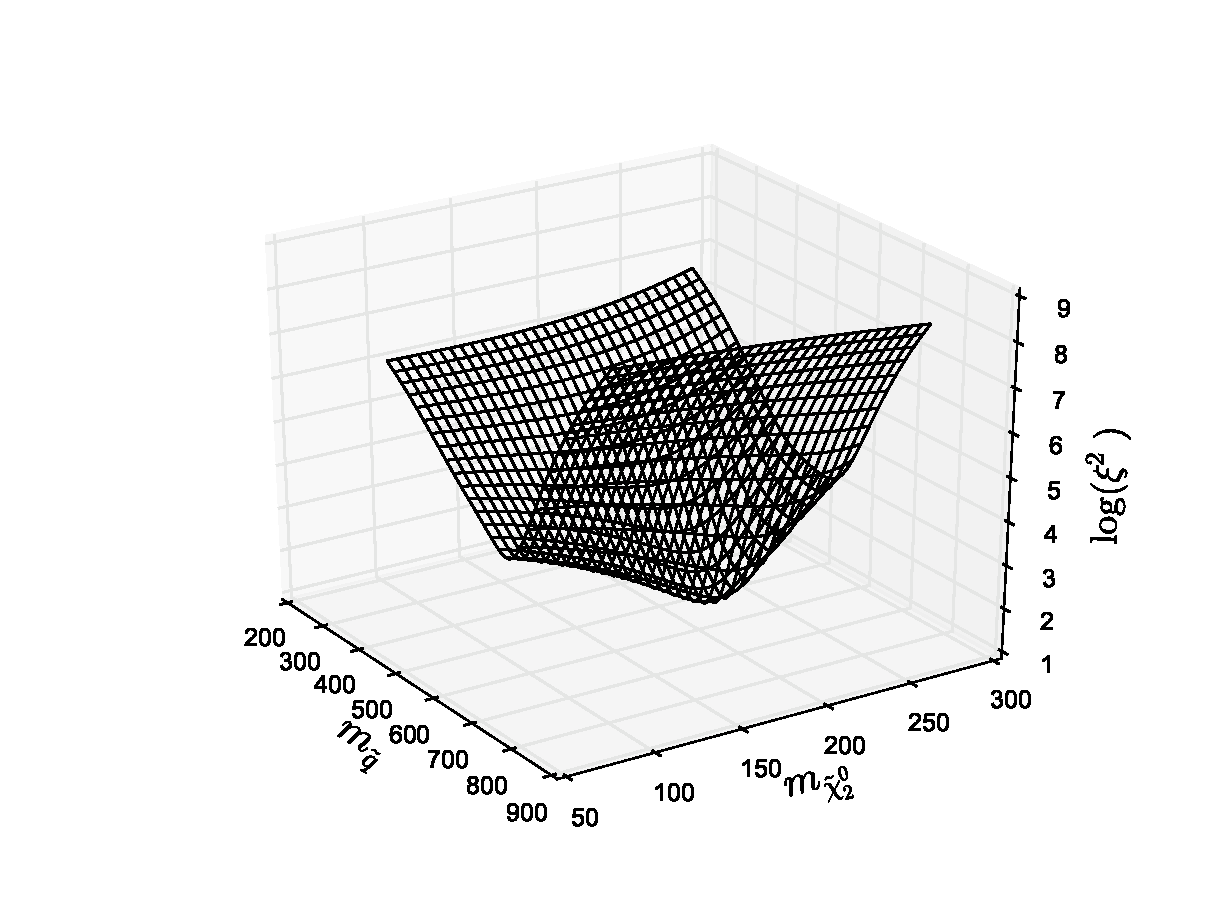
\includegraphics[width=\textwidth]{figures/3D_plot_xisquared_25_herwig_events_squark-chi2.pdf} 
		\caption{}
		\label{fig:3D_masses1}
	\end{subfigure}
	\begin{subfigure}[b]{0.49\textwidth}
		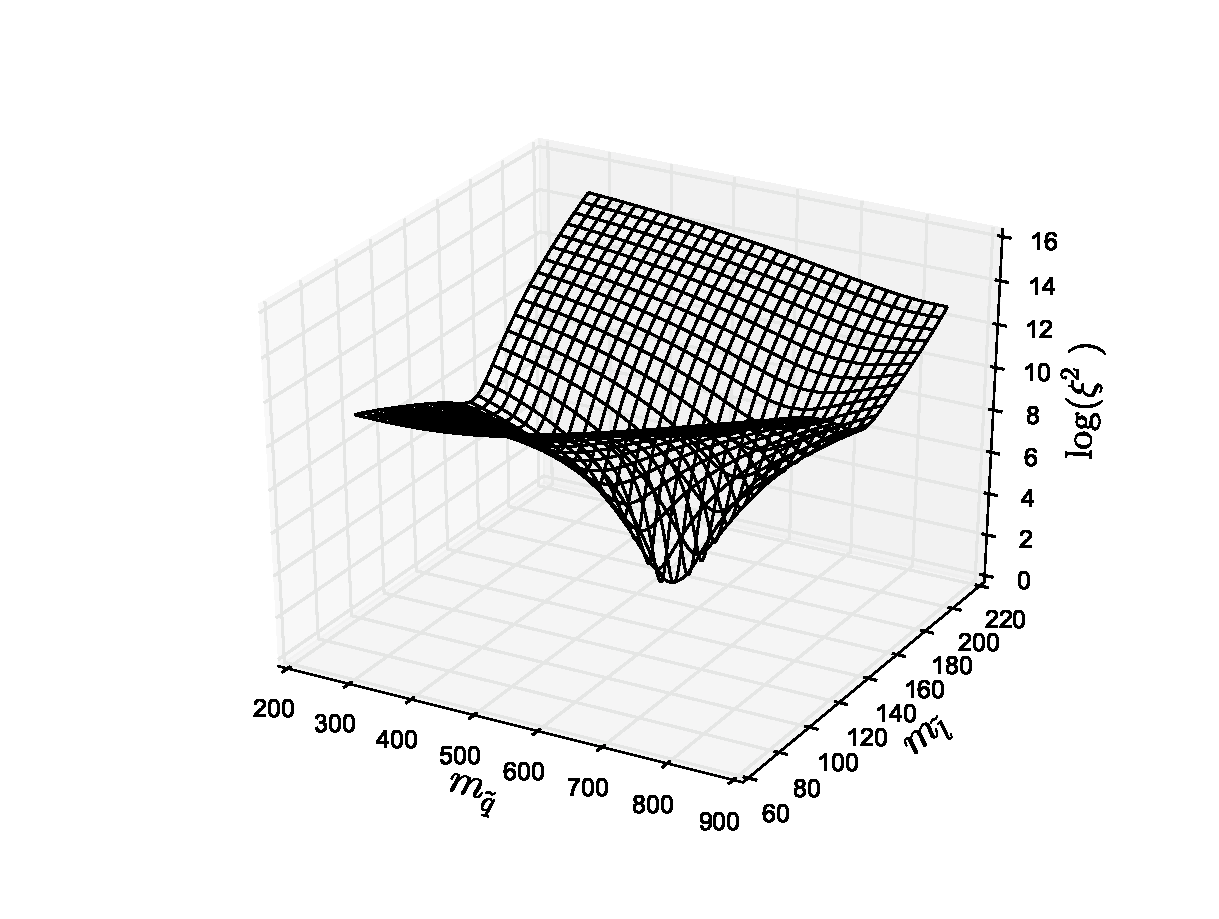
\includegraphics[width=\textwidth]{figures/3D_plot_xisquared_25_herwig_events_squark-slepton.pdf} 
		\caption{}
		\label{fig:3D_masses2}
	\end{subfigure}

	\begin{subfigure}[b]{0.49\textwidth}
		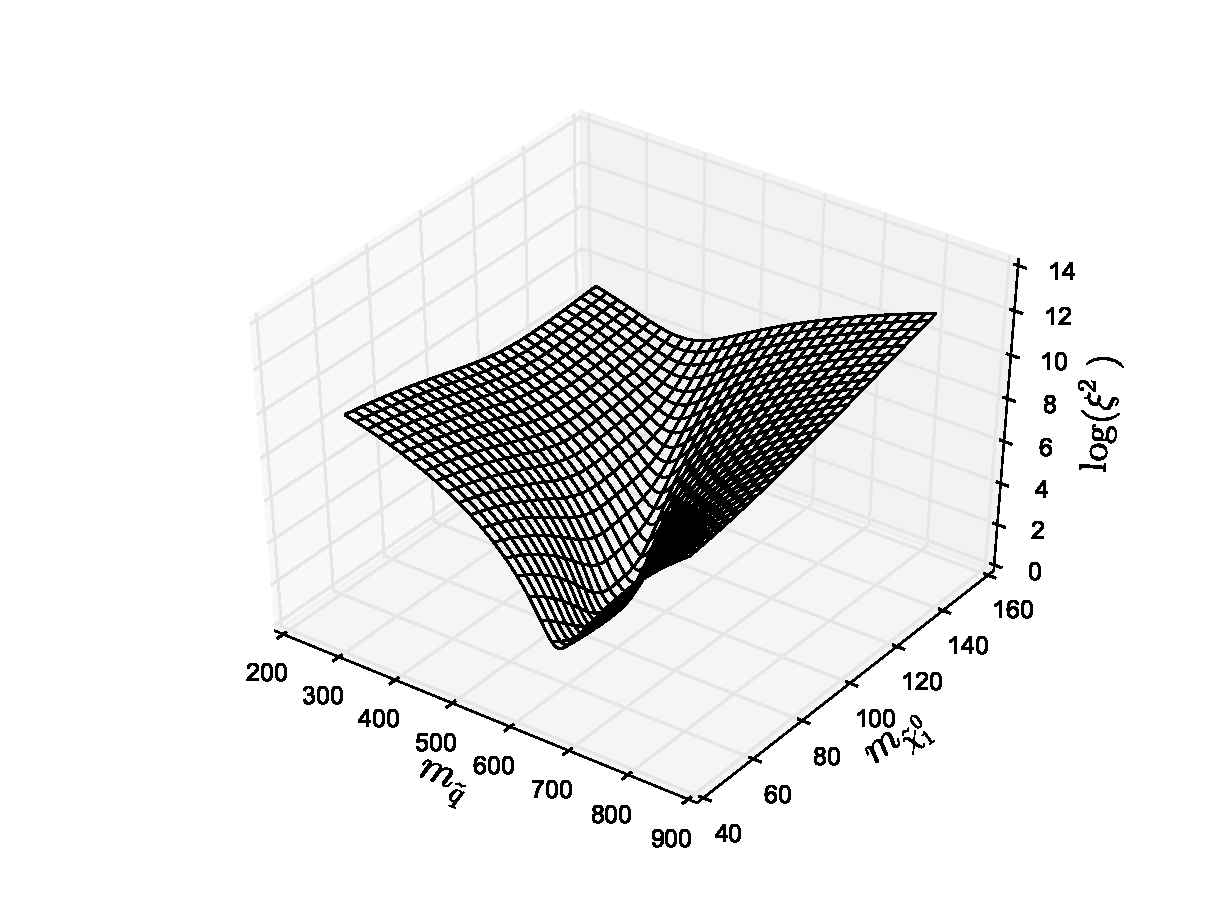
\includegraphics[width=\textwidth]{figures/3D_plot_xisquared_25_herwig_events_squark-chi1.pdf} 
		\caption{}
		\label{fig:3D_masses3}
	\end{subfigure}
	\begin{subfigure}[b]{0.49\textwidth}
		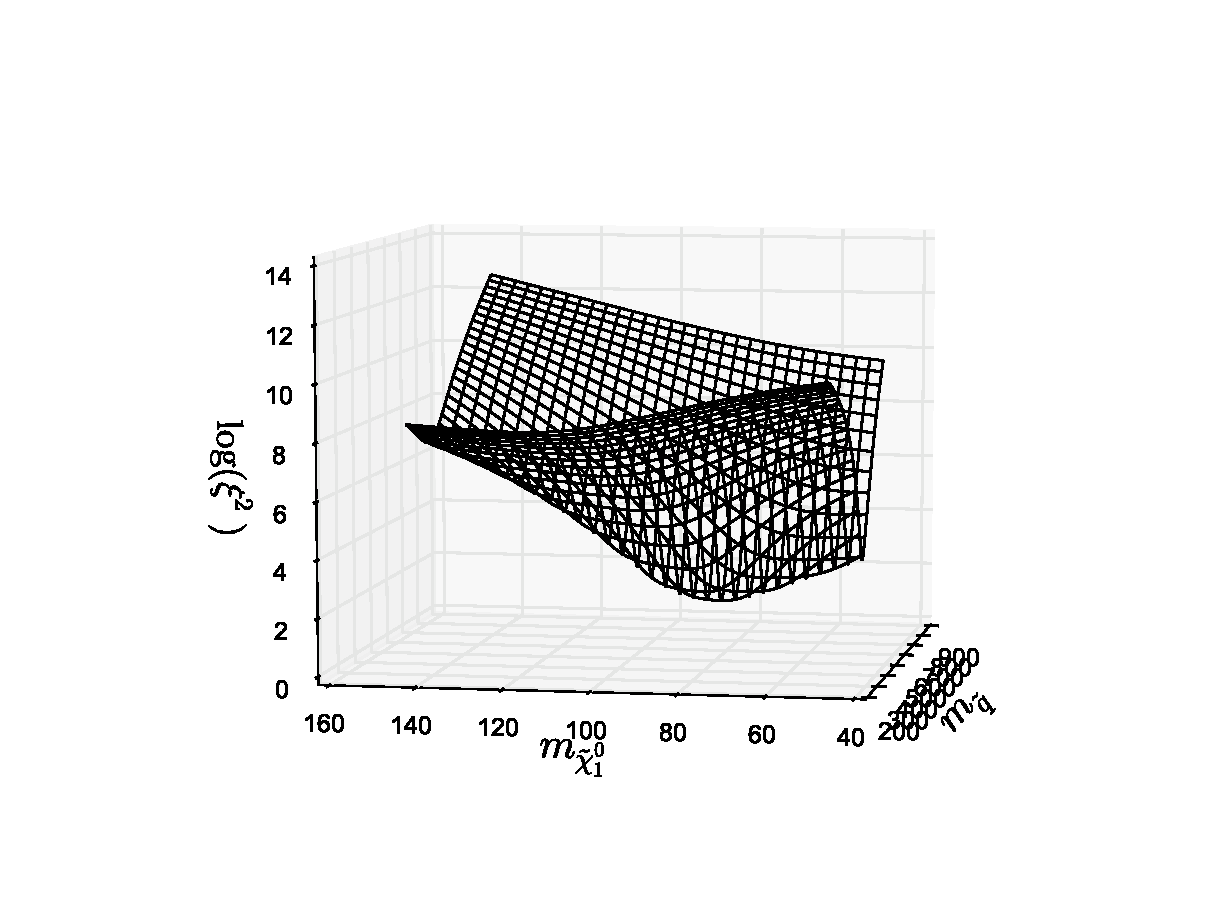
\includegraphics[width=\textwidth]{figures/3D_plot_xisquared_25_herwig_events_squark-chi1_rotated.pdf} 
		\caption{}
		\label{fig:3D_masses4}
	\end{subfigure}
	\caption{3D contour plot of $\log(\xi^2)$ in $m_{\tilde q}-m_i$ plane around the point of true minimum, where $i=\tilde \chi_2^0$ for (a), $i=\tilde l$ for (b) and $i=\tilde \chi_1^0$ for (c) and (d). The other two masses are fixed to their true value.}
	\label{fig:3D_masses}
\end{figure}



We begin by using the Minuit method Migrad to minimize the $\xi^2$ for 100 bins of 25 events each. A plot of the fit is shown in figure \ref{fig:herwig_migrad_nosmear_1p01} for an initial mass guess of 1.01 times the true mass values, and the best-fit points are summarized in table \ref{table:herwig_migrad_nosmear_1p01}. This is probably an unrealistically well-educated guess. Still, we see in the plot that many of the fit points to squark mass lie along a horizontal line. This happens when the minimizer is unable to find a better fit point than the initial guess. It is very difficult to find the optimal (and realistic?) tradeoff here, because the minimization is extremely sensitive to the initial guess -- if it is too far off, the minimization fails, and if it is too close it will end up choosing the initial value.

This leads us to investigate other minimization algorithms. We employ methods bundled in the Python package {\ttfamily Scipy} \cite{SciPy}. It features a minimization routine which contains as many as 12 different algorithms suitable for different purposes. The function we are minimizing is a quartic polynomial and thus differentiable. Also, we have bounds on the parameters since we know the masses should be positive. Hence we look at methods for minimizing differentiable functions over bounded areas. Two such methods are the {\it Truncated Newton algorithm/Newton Conjugate-Gradient (TNC)}\cite{Nash:1984} and {\it Sequential Least-Squares Programming (SLSQP)}\cite{Kraft:1988}. \marginpar{Say something about the actual mathematics of the two.} Figure \ref{fig:scipy_fit_nosmear} shows fits using these two methods. The performance is summarized in table \ref{table:herwig_scipy_comparison}. We see that the TNC method clearly seems to be performing better on our problem, so we will investigate further with this method. \marginpar{TODO: Do a minimization with x=1.0 initial mass guess, to see how well we possibly can do.}


\begin{figure}[hbt]
\centering
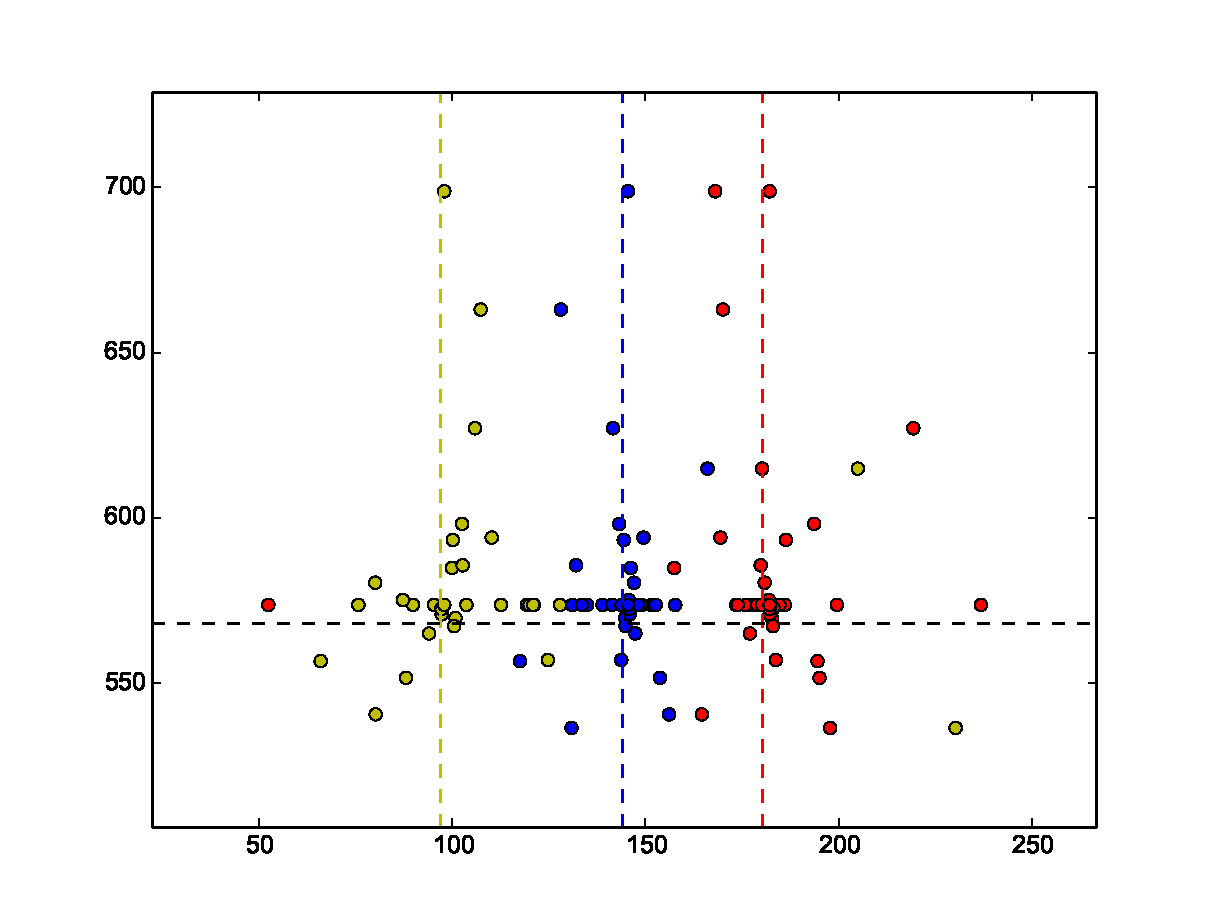
\includegraphics[scale=0.7]{figures/herwig_migrad_1p01_initial_guess_0p1_error.pdf} 
\caption{Best-fit points of 100 bins of 25 events generated with Herwig++, without momentum smearing and with no combinatorics, minimized using Migrad. The initial parameters given to Migrad are 1.01 times the true values for all four masses and the step size is 0.1 times the initial guess.}
\label{fig:herwig_migrad_nosmear_1p01}
\end{figure}



\begin{table}[hbt]
	\centering
	\begin{tabular}{| l | l | l | l | l |}
		\hline
		Particle 			& $\tilde q$	& $\tilde \chi_2^0$	& $\tilde l$	& $\tilde \chi_1^0$ \\ \hline
		True mass [GeV]		& 568 (average) & 180 				& 144 			& 97 				\\ \hline
		Migrad best-fit 	& $578 \pm 22 [24]$ 	& $181 \pm 15 [15]$ 	& $145 \pm 6 [6]$	& $101 \pm 19 [19]$ \\ \hline
	\end{tabular}
	\caption{Summary of Migrad fit to 25 event bins corresponding to figure \ref{fig:herwig_migrad_nosmear_1p01}.}
	\label{table:herwig_migrad_nosmear_1p01}
\end{table}

\begin{table}[hbt]
	\centering
	\begin{tabular}{| l | l | l | l | l |}
		\hline

		Particle   			& $\tilde q$ 	&$\tilde \chi_2^0$ 	& $\tilde l$ 	& $\tilde \chi_1^0$    	\\ \hline
		True mass [GeV]     & 568 (average) & 180				& 144			& 97					\\
		TNC, $x = 1.05$* &	$551 \pm 69 [71]$ & $179 \pm 18 [18]$ & $150 \pm 11 [12]$ & $111 \pm 23 [27]$ \\
		SLSQP, $x = 1.05$ &	$525 \pm 99 [108]$ & $176 \pm 26 [26]$ & $150 \pm 22 [23]$ & $114 \pm 38 [41]$ \\
		TNC, $x = 1.1$ &		$565 \pm 73 [73]$ & $184 \pm 25 [25]$ & $154 \pm 22 [24]$ & $114 \pm 24 [29]$ \\
		SLSQP, $x = 1.1$ &	$536 \pm 112 [116]$ & $193 \pm 92 [93]$ & $167 \pm 95 [97]$ & $133 \pm 103 [109]$ \\ \hline
	\end{tabular}
	\caption{Summary of TNC and SLSQP fits to 25 event bins corresponding to figure \ref{fig:scipy_fit_nosmear}. Fitted parameters are given as `average over bins $\pm$ empirical rms variation [true rms variation]'. The true rms variation means rms deviation from the true mass value. (*The given $x$ means $M_\mathrm{initial}= x M_\mathrm{true}$ for all unknown masses, $M_\mathrm{initial}$ being the starting point of the search.)}
	\label{table:herwig_scipy_comparison}
\end{table}


\begin{figure}[hbt]
	\centering
	\begin{subfigure}[b]{0.45\textwidth}
		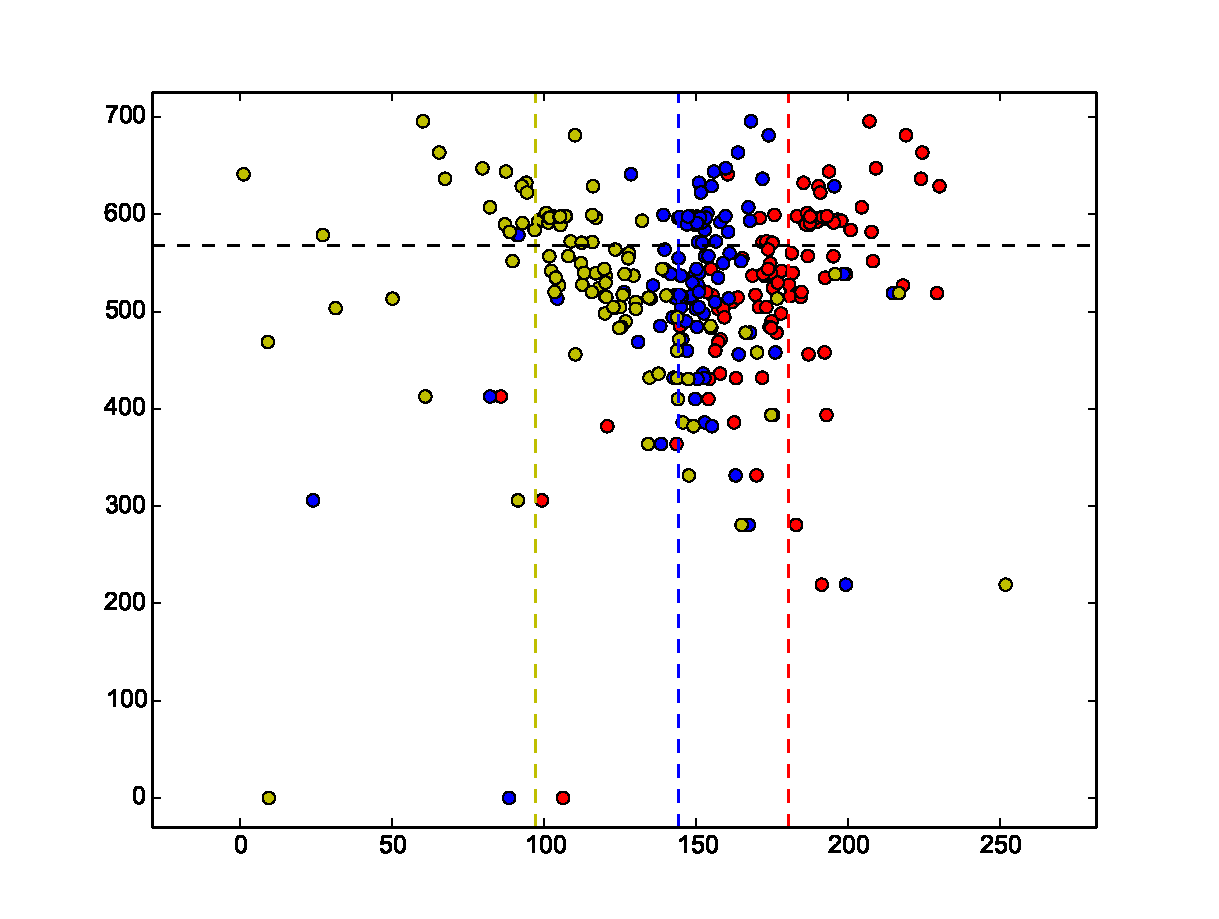
\includegraphics[width=\textwidth]{figures/herwig_scipy_slsqp_minimization_1p05_initial_guess.pdf} 
		\caption{}
		\label{fig:scipy_fit_nosmear1}
	\end{subfigure}
	\begin{subfigure}[b]{0.45\textwidth}
		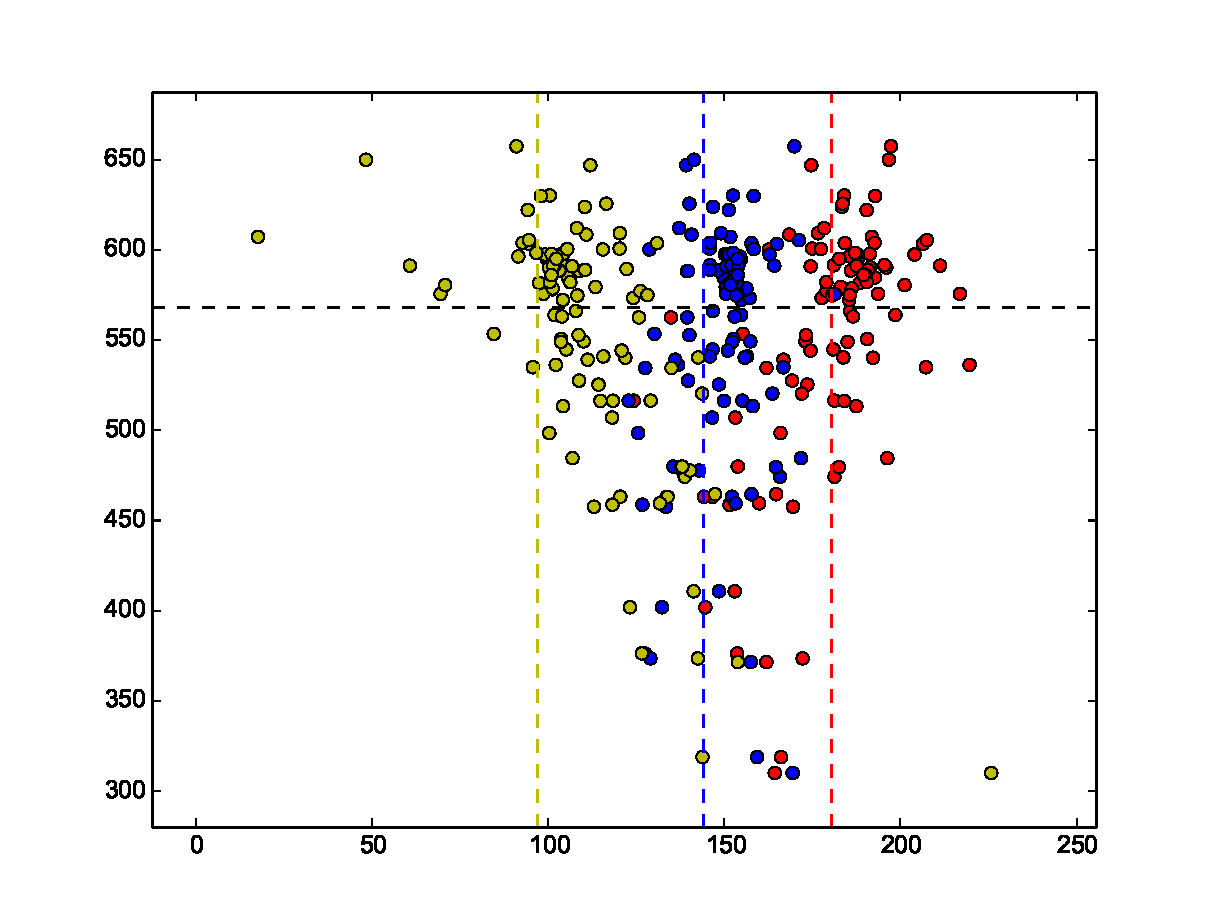
\includegraphics[width=\textwidth]{figures/herwig_scipy_tnc_minimization_1p05_initial_guess.pdf} 
		\caption{}
		\label{fig:scipy_fit_nosmear2}
	\end{subfigure}

	\begin{subfigure}[b]{0.45\textwidth}
		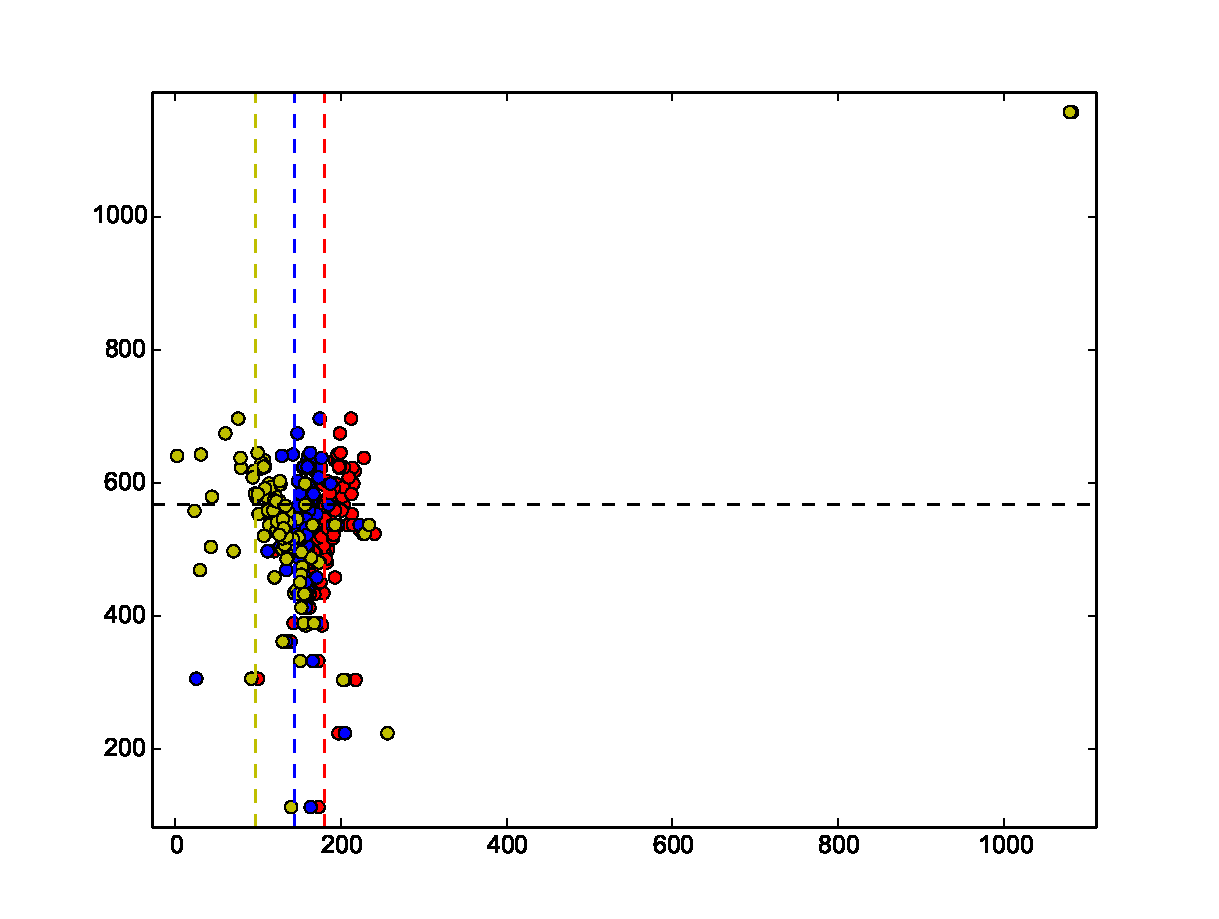
\includegraphics[width=\textwidth]{figures/herwig_scipy_slsqp_minimization_1p1_initial_guess.pdf} 
		\caption{}
		\label{fig:scipy_fit_nosmear3}
	\end{subfigure}
	\begin{subfigure}[b]{0.45\textwidth}
		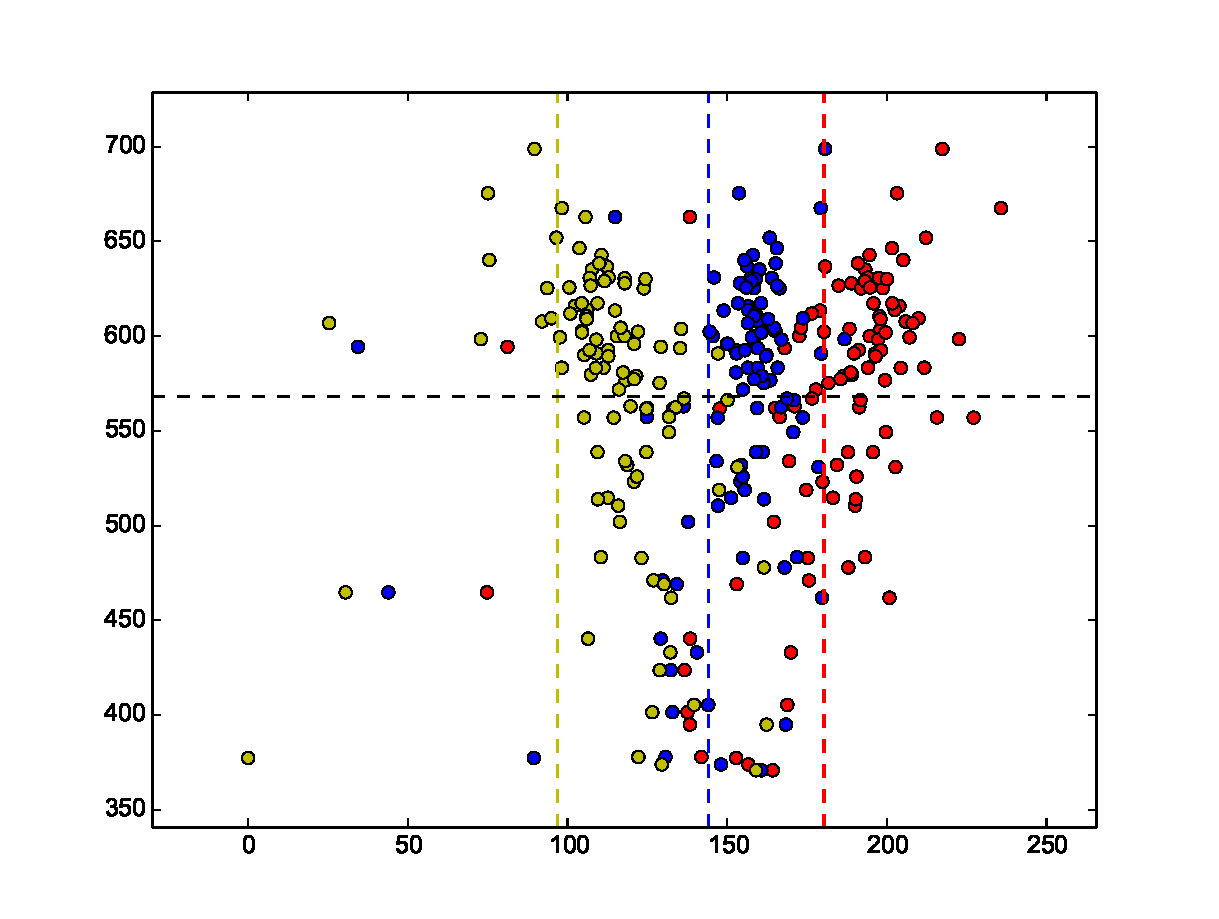
\includegraphics[width=\textwidth]{figures/herwig_scipy_tnc_minimization_1p1_initial_guess.pdf} 
		\caption{}
		\label{fig:scipy_fit_nosmear4}
	\end{subfigure}
	\caption{Best-fit points for 100 bins of 25 Herwig++ generated events for initial guesses of $1.05 M_\mathrm{true}$ ((a), (b)) and $1.1 M_\mathrm{true}$ ((c), (d)) using Newton Conjugate-Gradient (TNC) ((a),(c)) and sequential least squares (SLSQP) ((b), (d)) methods for minimization. The fits are summarized in table \ref{table:herwig_scipy_comparison}. Note that figure (c) has outliers stretching the axes, making it seem more clustered compared to the others than it is.}
	\label{fig:scipy_fit_nosmear}
\end{figure}



\section{Modelling the detector resolution by smearing momenta}
In a detector, the resolution with which we can measure momenta of the particles is limited. We model this limitation by smearing the particle momenta according to the formula 
\begin{align}
	\tilde{p}^\mu = p^\mu \left( 1 + r_n \frac{s}{\sqrt{E \mathrm{[GeV]}}} \right),\label{eq:smear1}
\end{align}
where $r_n$ is a standard normal-distributed random variable and $s$ is the chosen resolution. All components $\mu$ are smeared with the same $r_n$ such that the direction is not altered. The formula is taken from the {\ttfamily AcerDET} manual \cite{RichterWas:2002ch}. The manual prescribes different values of $s$ for different types of particles: 0.10 for photons, 0.12 for electrons and 0.50 or 1.00 for hadron jets ({\it i.e.\ } the quarks, in our case) depending on the pseudorapidity $|\eta|$ of the jet. \marginpar{Question to Are: The discrimination is given in terms of an AcerDET parameter called CALOTH -- I am guessing it stands for calorimeter threshold. What is a typical value? Is it the value 3.2 that is discussed in section 2.1 of the manual?}. Muons are smeared with a slightly different formula,
\begin{align}
	\tilde{p}^\mu = p^\mu / \left( 1 + r_n \cdot 0.005{\sqrt{p_T \mathrm{[GeV]}}} \right),\label{eq:smear2}
\end{align}
\marginpar{Question to Are: Should it really be division in this formula, or is it a typo in AcerDET manual?} where $p_T$ is the transverse momentum of the muon.

% Old:
% The first complication we add is that of momentum smearing. This is done to model the uncertainties that stem from the detectors. According to the prescription from the {\ttfamily AcerDET} manual \cite{RichterWas:2002ch} we use a smearing of the form
% \begin{align}
% 	\tilde{p}^\mu = p^\mu \left( 1 + r_n \frac{s}{\sqrt{E \mathrm{[GeV]}}} \right),\label{eq:smear}
% \end{align}
% where $r_n$ is a standard normal-distributed random variable and $s$ is the chosen smearing resolution. All components $\mu$ are smeared with the same $r_n$ such that the direction is not altered.\marginpar{TODO: Differentiate between types of particles, give different amounts of smearing. See AcerDET manual.} Table \ref{table:fit_smear} shows best-fit results for 10 \% and 30 \% smearing. We see that still the error, even at 30 \% smearing, are of the order of a few percent -- except for the lightest neutralino, where it is 32 \% off. It appears that the relative fit error increases with decreasing sparticle mass. This might indicate that {\ttfamily SIMPLEX} fits all masses with about the same absolute error -- which would make the relative error larger for smaller sparticle mass. The dilepton invariant mass distribution is shown again for the two smearing choices in figure \ref{fig:dilepton_invariant_mass_smearing}.

% \begin{table}[hbt]
% 	\centering
% 	\begin{tabular}{| l | l | l | l | l | l |}
% 		\hline
% 		Smearing resolution &					&  $m_{\tilde{q}}$ & $m_{\tilde{\chi}_2^0}$ & $m_{\tilde{l}}$ & $m_{\tilde{\chi}_1^0}$ \\ \hline
% 							& True values [GeV] 	& 545.4 & 180.3 & 144.1 & 97.0 \\ \hline
% 		10 \% 				& Best-fit values [GeV] & 547.0 & 185.5 & 149.8 & 103.1 \\ \hline
% 		10 \% 				& Relative fit error  & 0.3 \% & 2.8 \% & 4.0 \% & 6.3 \% \\ \hline
% 		30 \% 				& Best-fit values [GeV] & 565.4 & 177.7 & 135.2 & 65.8 \\ \hline
% 		30 \% 				& Relative fit error  & 3.7 \% & 1.5 \% & 6.1 \% & 32.2 \% \\ \hline
% 	\end{tabular}
% 	\caption{SIMPLEX fit of 1000 events with momentum smearing.}
% 	\label{table:fit_smear}
% \end{table}

% \begin{figure}[hbt]
% 	\centering
% 	\begin{subfigure}[b]{0.4\textwidth}
% 		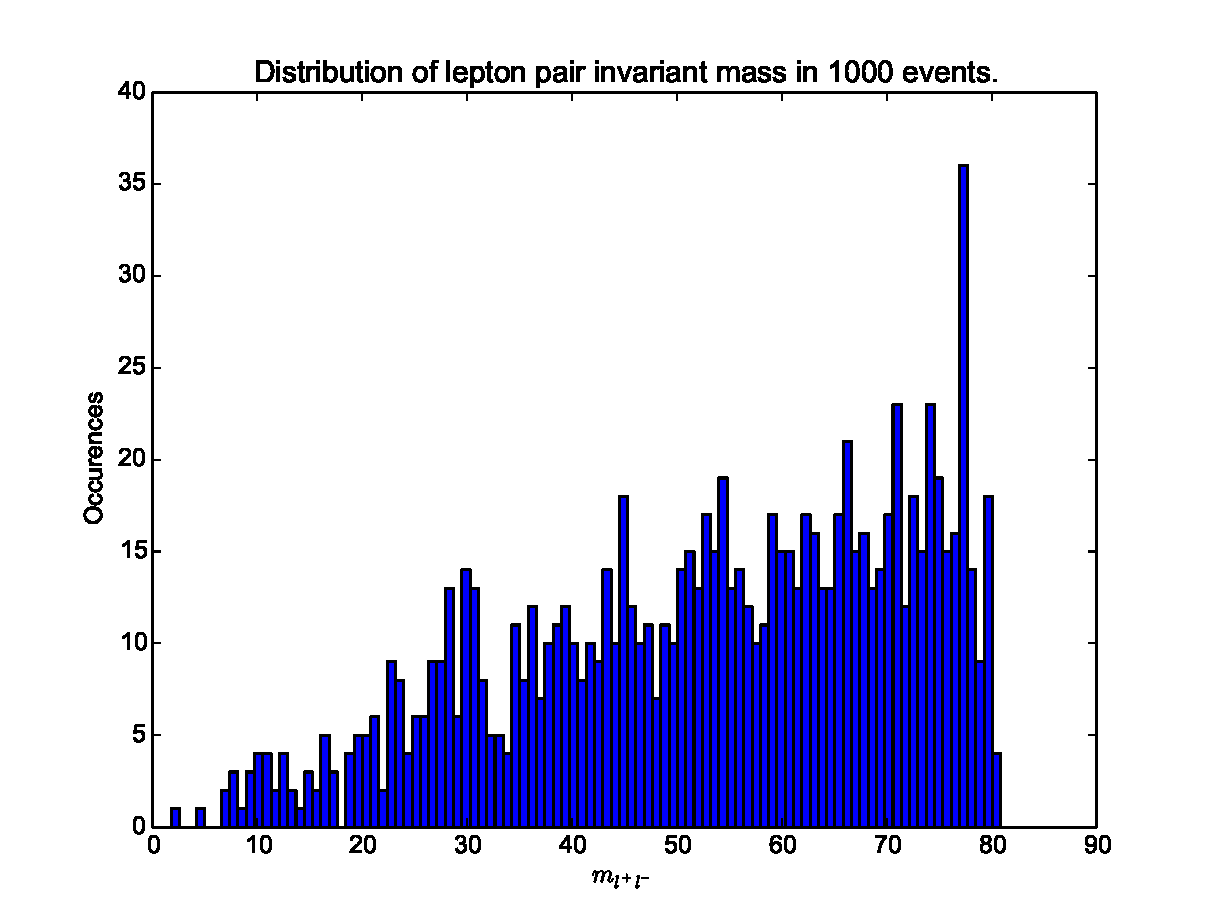
\includegraphics[width=\textwidth]{figures/dilepton_invariant_mass_comphep-data_smearing-0point1_events-1000.pdf} 
% 		\caption{ }
% 	\end{subfigure}
% 	\begin{subfigure}[b]{0.4\textwidth}
% 		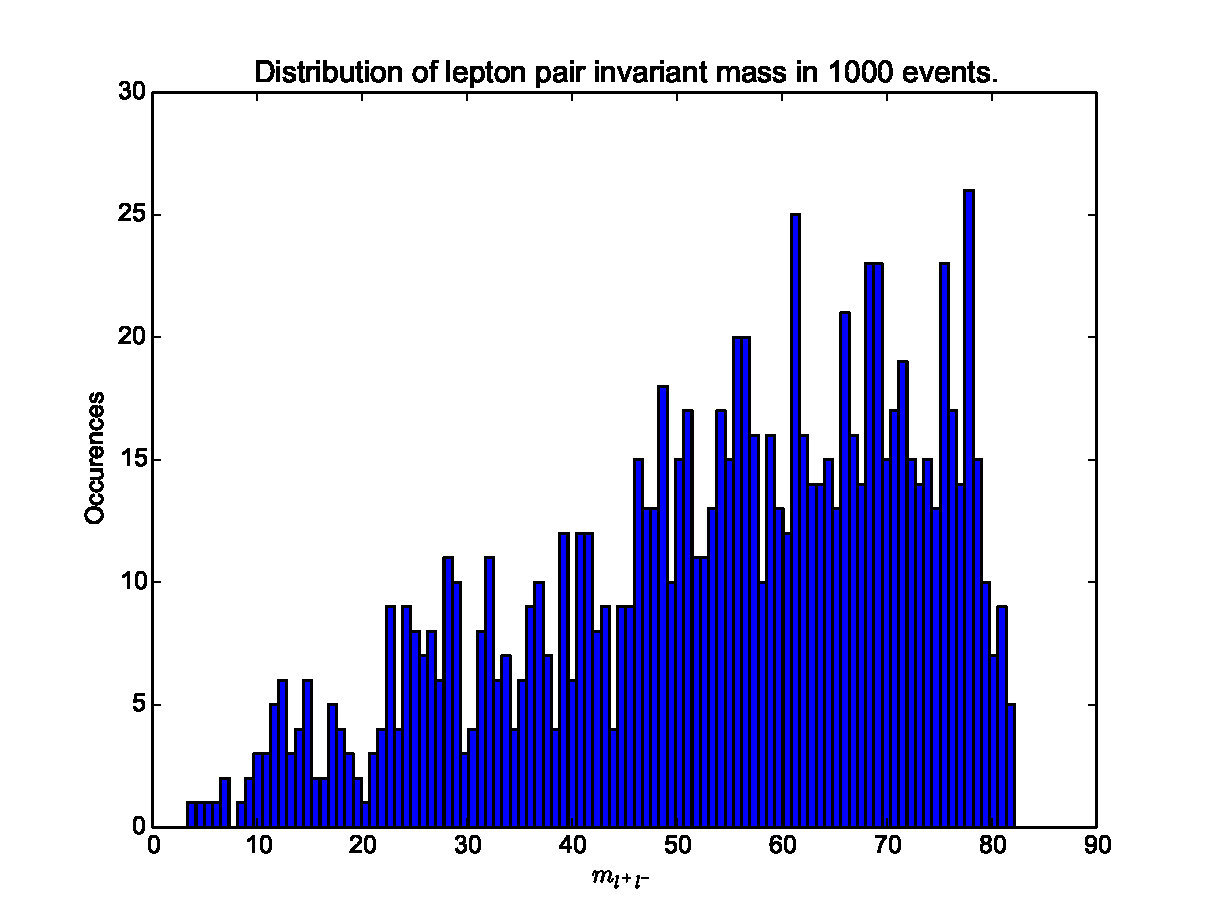
\includegraphics[width=\textwidth]{figures/dilepton_invariant_mass_comphep-data_smearing-0point3_events-1000.pdf}
% 		\caption{ } 
% 	\end{subfigure}
% 	\caption{Dilepton invariant mass distribution with 10 \% (a) and 30 \% (b) momentum smearing.}
% 	\label{fig:dilepton_invariant_mass_smearing}
% \end{figure}


\subsection{How does matrix invertibility depend on smearing?}
Given a 4-momentum vector $p^\mu_i$, what are its statistical properties after smearing with the prescription in Eq. \eqref{eq:smear1}? The stochastic variable $r_n$ in \eqref{eq:smear1} is drawn from a standard normal distribution, {\it e.g.}\
\begin{align}
	r_n \sim N(\mu,\sigma) = N(0,1),
\end{align}
where $N$ denotes a normal distribution, $\mu$ is the expectation value and $\sigma$ is the standard deviation. From basic probability theory we know that for expectation values $\mathrm E(X)$ and variances $\mathrm{Var}(X)$ we have
\begin{align}
	\mathrm E(aX+bY) = a\mathrm E(X) + b\mathrm E(Y),\\
	\mathrm{Var}(aX + bY) = a^2\mathrm{Var}(X) + b^2\mathrm{Var}(Y).\nonumber
\end{align}
Thus for a smeared 4-vector $\tilde{p}^\mu_i$ we have
\begin{align}
	\mathrm E(\tilde{p}^\mu_i) = p^\mu_i,\\
	\mathrm{Var}(\tilde{p}^\mu_i) = \frac{s^2 (p^\mu_i)^2}{E_i\mathrm{[GeV]}}.
\end{align}
For a sum of smeared 4-vectors we thus get
\begin{align}
		\mathrm E\left(\sum_i \tilde{p}^\mu_i\right) = \sum_i p^\mu_i,\\
	\mathrm{Var}\left(\sum_i \tilde{p}^\mu_i\right) = \sum_i \frac{s^2 (p^\mu_i)^2}{E_i\mathrm{[GeV]}}.
\end{align}

\marginpar{TODO: Look at the analytical expressions for det(A), E(det(A)) and Var(det(A)) as a function of smearing, with the redefinitions in the next section for A4 / A8. Maybe use Mathematica to calculate?}



\section{Taking combinatorial issues into account}
In a real detector event, we will not have information about which of the measured particles belong to which chain. Therefore we must evaluate all allowed combinations and see which appears most likely to be the correct one. We have two possible cases, depending on whether the OSSF leptons on the two sides are of the same or different generations: If all four leptons are the same, then there are 16 possible combinations including the two-fold ambiguity in the quark assignments, while the number reduces to eight if the leptons come in two different generations. 

{\it -- What are the relative branchings to the two cases? Does it make sense to discard the all-leptons-equal events like Webber does or do we lose a lot of events? Answer: The branching is of course 50-50, since the branching from neutralino2 is equal to both leptons. The plan is therefore to implement combinatorics for the most general case, possibly with a switch option to reduce to unequal sides for comparison.}










%%%%%%%%%%%%%%%%%%%%%%%%%%%%%%%%%%%%%%%%
\chapter{Improvements of the method}
%%%%%%%%%%%%%%%%%%%%%%%%%%%%%%%%%%%%%%%
To think about: How do we scan when we don't know true values? The fit is sensitive to initial values. Might it be fruitful to run many minimizations with different starting positions? That would essentially stack another 4-dimensional minimization on top of this one. Would scale CPU time enormously. Probably not that clever.




\appendix

\chapter{Algorithms}

\section{On-shell two-body decay}
\label{sec:decayalgorithm}
 The particles will go back-to-back in the rest frame of the decaying particle - the direction is drawn randomly from a uniform spherical distribution. This can be achieved in spherical coordinates by the assignments
\begin{align}
	U, V &= \text{uniform}(0,1)\nonumber \\
	\phi &= 2\pi U\\
	\theta &= \arccos(2V-1) \nonumber
\end{align}
The decay algorithm, in python notation, is as follows. Particle 1 of 4-momentum $p_1$ decays to particle 2 and 3 of 4-momentum $p_2$ and $p_3$. 
\begin{lstlisting}
	p1abs = sqrt( float( dot( p1 , transpose(p1) ) ) )  # 3-momentum of particle 1 in lab frame

	# == Kinematical decay in RF of particle 1 ==
	# Primed coordinates are in RF of particle 1
	p2absprime = 1.0/(2*m1) * sqrt( (m1**2-m2**2-m3**2)**2- 4*m2**2*m3**2 ) # abs-val of 3-momentum of particle 2/3 in RF of particle 1

	# Random point picking on a sphere
	U, V = random.uniform(0,1,2) 
	phi = 2*pi*U 				  
	theta = arccos(2*V-1) 		 

	# Calculate cartesian 3- and 4-momentum of particle 2&3
	p2prime = matrix([ p2absprime*sin(theta)*cos(phi) , 
					   p2absprime*sin(theta)*sin(phi) , 
				   	   p2absprime*cos(theta) ])
	p3prime = -p2prime
	E2prime = sqrt( p2absprime**2 + m2**2 )
	E3prime = sqrt( p2absprime**2 + m3**2 )
	P2prime = matrix([ E2prime , p2prime[0,0] , p2prime[0,1] , p2prime[0,2] ])
	P3prime = matrix([ E3prime , p3prime[0,0] , p3prime[0,1] , p3prime[0,2] ])

	# == Back-transform to lab frame ==
	# First check whether it is necessary to boost
	if p1abs > 1e-10:

		# Lorentz boost along x-direction to get to rotated lab frame
		# (lab frame moves in negative x direction)
	 	vlab = -p1abs/sqrt(p1abs**2 + m1**2) # velocity of particle 1 in lab frame
		gamma = 1/sqrt(1-vlab**2)

		P2rot = matrix([ gamma*(P2prime[0,0] - vlab*P2prime[0,1]) , 
				      gamma*(P2prime[0,1] - vlab*P2prime[0,0]) ,
				      P2prime[0,2] , P2prime[0,3] ])
		P3rot = matrix([ gamma*(P3prime[0,0] - vlab*P3prime[0,1]) , 
				      gamma*(P3prime[0,1] - vlab*P3prime[0,0]) ,
				      P3prime[0,2] , P3prime[0,3] ])

		# == Rotate back to lab frame ==

		# Calculate the unit vectors of the rotated system axes in terms of lab axes

		# The definition is that x axis is along p1.
		# For the other axes we must make a choice - y&z directions are undetermined,
		# only the yz plane is determined from x choice. But since we have drawn 
		# random angles and the yz plane is not boosted, the choice does not matter
		# as long as we are consistent from event to event.
		# So we pick two vectors orthogonal to p1 and do Gram-Schmidt orthogonalization:
		v1 = p1
		v2 = matrix([ p1[0,1] , -p1[0,0] , 0 ])
		v3 = matrix([ p1[0,2] , 0 , -p1[0,0] ])

		u1 = v1
		u2 = v2 - proj(v2,u1)
		u3 = v3 - proj(v3,u1) - proj(v3,u2)

		xrot = u1/linalg.norm(u1)
		yrot = u2/linalg.norm(u2)
		zrot = u3/linalg.norm(u3)

		# Form a matrix T which takes a vector in the lab basis to a vector 
		# in the rotated basis by
		T = concatenate( (xrot , yrot , zrot) , axis=0 )
		# What we need is to rotate from rotated basis to lab basis, so we need the inverse
		# - which is the transpose, since rotation matrices are orthogonal. 
		# Also, to ease calculation, we let T be the 3x3 submatrix of T4, setting the [0,0]
		# component of T4 to 1 to leave time component invariant under this spatial rotation
		T4 = matrix([[1,     0,     0,    0],
						[0,T[0,0],T[0,1],T[0,2]],
						[0,T[1,0],T[1,1],T[1,2]],
						[0,T[2,0],T[2,1],T[2,2]] ])

		P2 = T4.T*P2rot.T
		P3 = T4.T*P3rot.T
		P2 = P2.T
		P3 = P3.T

	# If it was unneccessary, i.e. decay happened in lab frame, then
	else:
		P2 = P2prime
		P3 = P3prime
\end{lstlisting}






\bibliographystyle{plain}
\bibliography{thesis-bibliography}

\end{document}